\chapter{Evaluation} \label{chap:evaluation}

\section*{}

\minitoc \mtcskip \noindent
This section evaluates how the solution developed proves the hypothesis proposed in \sectionintroref{sec:main_hypothesis} and fulfills the requirements presented in \sectionintroref{sec:desiderata}. \sectionintroref{sec:scenarios_experiments} proposes scenarios and experiments that will be used to evaluate the developed solution. \sectionintroref{sec:evaluation_discussion} discusses the results of the experiments and concludes the fulfillment of the requirement each test aims to assess. \sectionintroref{sec:evaluation_hypothesis} verifies if the main hypothesis is proved with the evaluation data. Finally, \sectionintroref{sec:evaluation_lessons_learned} reflects on the lessons learned during the evaluation process. 

\section{Scenarios and Experiments}\label{sec:scenarios_experiments}

To validate to which extent we were able to reach the aforementioned goals (\cf Section~\ref{sec:motivation}), we proceed to evaluate our architecture and implementation \textit{proof-of-concept} in both virtual --- using Docker with an Unix-compatible version of MicroPython --- and physical setups --- using both ESP8266 and ESP32 connected in the same Wi-Fi network.

\begin{description}
    \item[\textbf{ES1}] A room has 3 sensors that give temperature and humidity readings every minute. There is a virtual sensor that compares the results (of both temperature and humidity) and triggers depending on the configured thresholds. An AC unit must be provided with the comparison result to define both (a) if it \textit{switches on/off}, and (b) its operating mode: \textit{cool}, \textit{heat}, and \textit{dehumidify}. The Minimal Working System (MWS) consists in (a) one temperature sensor, (b) one humidity sensor, (c) one \textit{node} capable of making the decision, and (d) working communication channels amongst them.
    \item[\textbf{ES2}] A system contains 20 devices that are responsible for propagating an injected message to their output. In the end, the injected message must reach an output MQTT topic.
\end{description}

\begin{figure}[h]
\centering
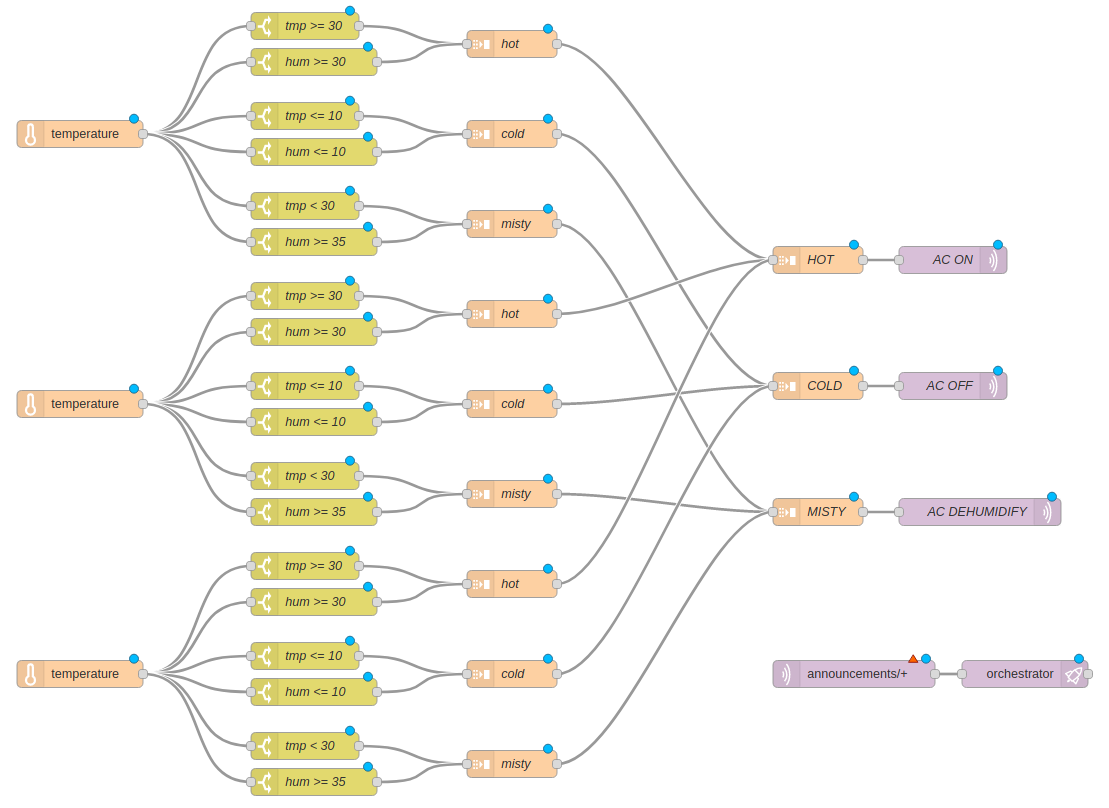
\includegraphics[width=\textwidth]{scenario1.png}
\caption[Node-RED implementation of scenario 1]{Node-RED implementation of scenario 1}\label{fig:scenario1_node_red}
\end{figure}

\textbf{ES1}, which resembles to a real-world scenario, aims to test the features of the developed solution with a moderately simple Node-RED \textit{flow} \seefigureref{fig:scenario1_node_red}, taking advantage of the \textit{nodes} developed for MicroPython code generation support. As complement, \textbf{ES2} allows the comparison of the developed solution to the already existing ones.

For each one of the experimental scenarios (\ie \textbf{ES1} and \textbf{ES2}) we defined a set of experimental tasks. 

For \textbf{ES1} two Sanity Checks were performed, one over virtual devices --- Sanity Check 1 (\textbf{ES1-SC1}) --- and other with physical devices --- Sanity Check 2 (\textbf{ES1-SC2}). A set of readings and message forwarding tasks were performed with no compensation or any other fault-tolerance strategy. Each sensor device only provides environmental readings to the system. Orchestration is centralized. We expect all round-trips to take less than the smallest part that can be resolved (measurement capability, which we estimate to be $<1$ second).

We further defined a set of (re-)orchestration experiments for \textbf{ES1}, where the system must allocate computation tasks among the available resources (\ie devices), namely:
\begin{description}
    \item[ES1-A] Minimal Working System (MWS) is achieved via multiple possible configurations by selective (provoked) device failure (fail-stop) using only virtual devices (\ie Docker);
    \item[ES1-B] MWS is achieved via multiple possible configurations by selective (provoked) device failure (fail-stop) using physical devices;
    \item[ES1-C] Inconsistent device behaviour, \eg appear and disappear in shorter intervals lower that the time needed for orchestrating convergence (OCT), that leads to activity impacting the MWS;
    \item[ES1-D] With 20 devices, each one with different processing capabilities. During orchestration, some devices will develop an out-of-memory error because they can't process all the processing tasks assigned to them, specifically the size of the script given. The orchestrator decides to send less tasks to these devices. The system will converge in a working solution. \textit{This scenario will be implemented with a modified device script. When devices receive a script, it will generate a memory error if the length of the script passes a certain threshold. This simulates the memory constraints of devices when receiving a file to big.}
    \item[ES1-E] With 20 devices, some of them have a memory leak with an unknown cause. After random time \texttt{Random(t0,t1)}, these problematic devices stop working with an out-of-memory error. The orchestrator thinks that the devices can't handle the quantity of processing tasks assigned to them, so in the re-orchestration it will assign fewer tasks. Since these devices will always break, the orchestrator will eventually not consider these devices in the assignment of nodes. \textit{This scenario will be implemented with a modified device script that will trigger an out-of-memory error after a random period after executing the given tasks.}
    \item[ES1-F] With 20 devices, there is a device that is sensitive to a particular \textit{node}, which causes the device to give out an out-of-memory error. The orchestrator will potentially assign this \textit{node} to the specific device. When the device gives out the out-of-memory error, the orchestrator will eventually converge in a solution where the \textit{node} is not assigned to the particular device, and the system will converge.  \textit{These out-of-memory errors will be simulated with the use of a failure \textit{node} that forces an \texttt{MemoryException} in the device.}
    \item[ES1-G] With 50 devices, each second the device has a probability to fail. This failure can go from 0 to 10 seconds, randomly chosen. The orchestrator must deal with the random failure of the devices and re-orchestrate the system. This experiment is considered a stress test, causing repeated failures and forcing constant re-orchestration.
\end{description}

With this set of experiments we can verify that the following constraints are meet:
\begin{enumerate}
    \item \textbf{Restrictions (predicates) are enforced.} Check that possible configurations lead to solutions that enforce defined predicates;
        \begin{enumerate}
            \item Temperature and humidity might coexist in the same, or in dedicated, devices;
        \end{enumerate}
    \item \textbf{Priorities are honored.} Check that all specified priorities were taken into account, and only violated if necessary;
        \begin{enumerate}
            \item Priority is given to edge devices, but fog and cloud can be used;
            \item Priority is given to the maximum level of decentralization, but some centralization can be used.
        \end{enumerate}
\end{enumerate}


Regarding \textbf{ES2}, a total of 20 devices where connected in a line topology, where a message is sent to a starting device which will propagate it to its output. All the devices implement this propagation logic, resulting in the initial message reaching the end of the line. The propagation time is measured, starting when the message is sent and ending when the message reaches the last node. This scenario was implemented with different experimental configurations, namely:
\begin{description}
    \item[ES2-A] Non-modified version of Node-RED, using the default \textit{node}-to-\textit{node} communication channel (\texttt{EventEmitter}), with all the nodes sharing the same run-time.
    
    \item[ES2-B] Modified version of Node-RED that uses MQTT as the \textit{node}-to-\textit{node} communication channel, with all the nodes sharing the same run-time.
    
    \item[ES2-C] MQTT-based modified Node-RED, where each \textit{node} of the \textit{flow} is assigned to a different virtual device (\ie a MicroPython-running Docker instance). The Docker instances and MQTT broker run in the same host machine.
    
    \item[ES2-D] MQTT-based modified Node-RED, where each \textit{node} of the \textit{flow} is assigned to a different virtual device. The Docker instances share one host, but the MQTT broker is in a different one. All parts are connected to the same Wi-Fi network.
    
    \item[ES2-E] Each physical device runs a simple script that performs the wanted behaviour, on top of a non-modified MicroPython firmware image, communicating with which other over MQTT. Node-RED is not used and there is no orchestration being performed.

    \item[ES2-F] MQTT-based modified Node-RED, along with the modified MicroPython firmware running on physical devices. Each each \textit{node} of the \textit{flow} is assigned to a different device, that are connected to the same WiFi network and communicate using MQTT between them. 
\end{description}

%%%%%%%%%%%%%%%%%%%%%%%%%%%% DISCUSSION %%%%%%%%%%%%%%%%%%%%%%%%%%%%%%%%%%%

\section{Discussion}\label{sec:evaluation_discussion}

The scenarios and respective experimental tasks were performed and several metrics of the system were measured. The following paragraphs present and discuss the experimental results.

\subsection{ES1: Sanity Checks}\label{sec:discussion_scenario1}

As mentioned previously (\cf \seesectionref{sec:scenarios_experiments}), the first scenario consists of a system that controls an A/C. This system takes into account readings of 3 temperature and humidity sensors to define if the room's temperature is too hot, cold of humid and sends commands to the A/C with the respective actions.

These experiments will prove that the devices can satisfy the \textit{nodes}, meaning that the system works as intended once the assignment is complete. With this premise, this will not verified again in the remaining experiments.

%%%%%%%%%%%%%%%%%%%%%% SC %%%%%%%%%%%%%%%%%%%%%%

\subsubsection{ES1-SC1}\label{sec:sanity_check_exp}

With the purpose of testing the overall functionality of the approach in a controlled way (the use of virtual devices reduce the proneness to hardware-provoked failures), the experiment resulting orchestration can be observed in \figureref{fig:sanity_check_graph}, where the \textit{Orchestrator node} allocated nine \textit{nodes} to each device. \figureref{fig:sanity_check_node_assignment_visual} demonstrates in which devices each \textit{node} was assigned to.

\begin{figure}[h]
\centering
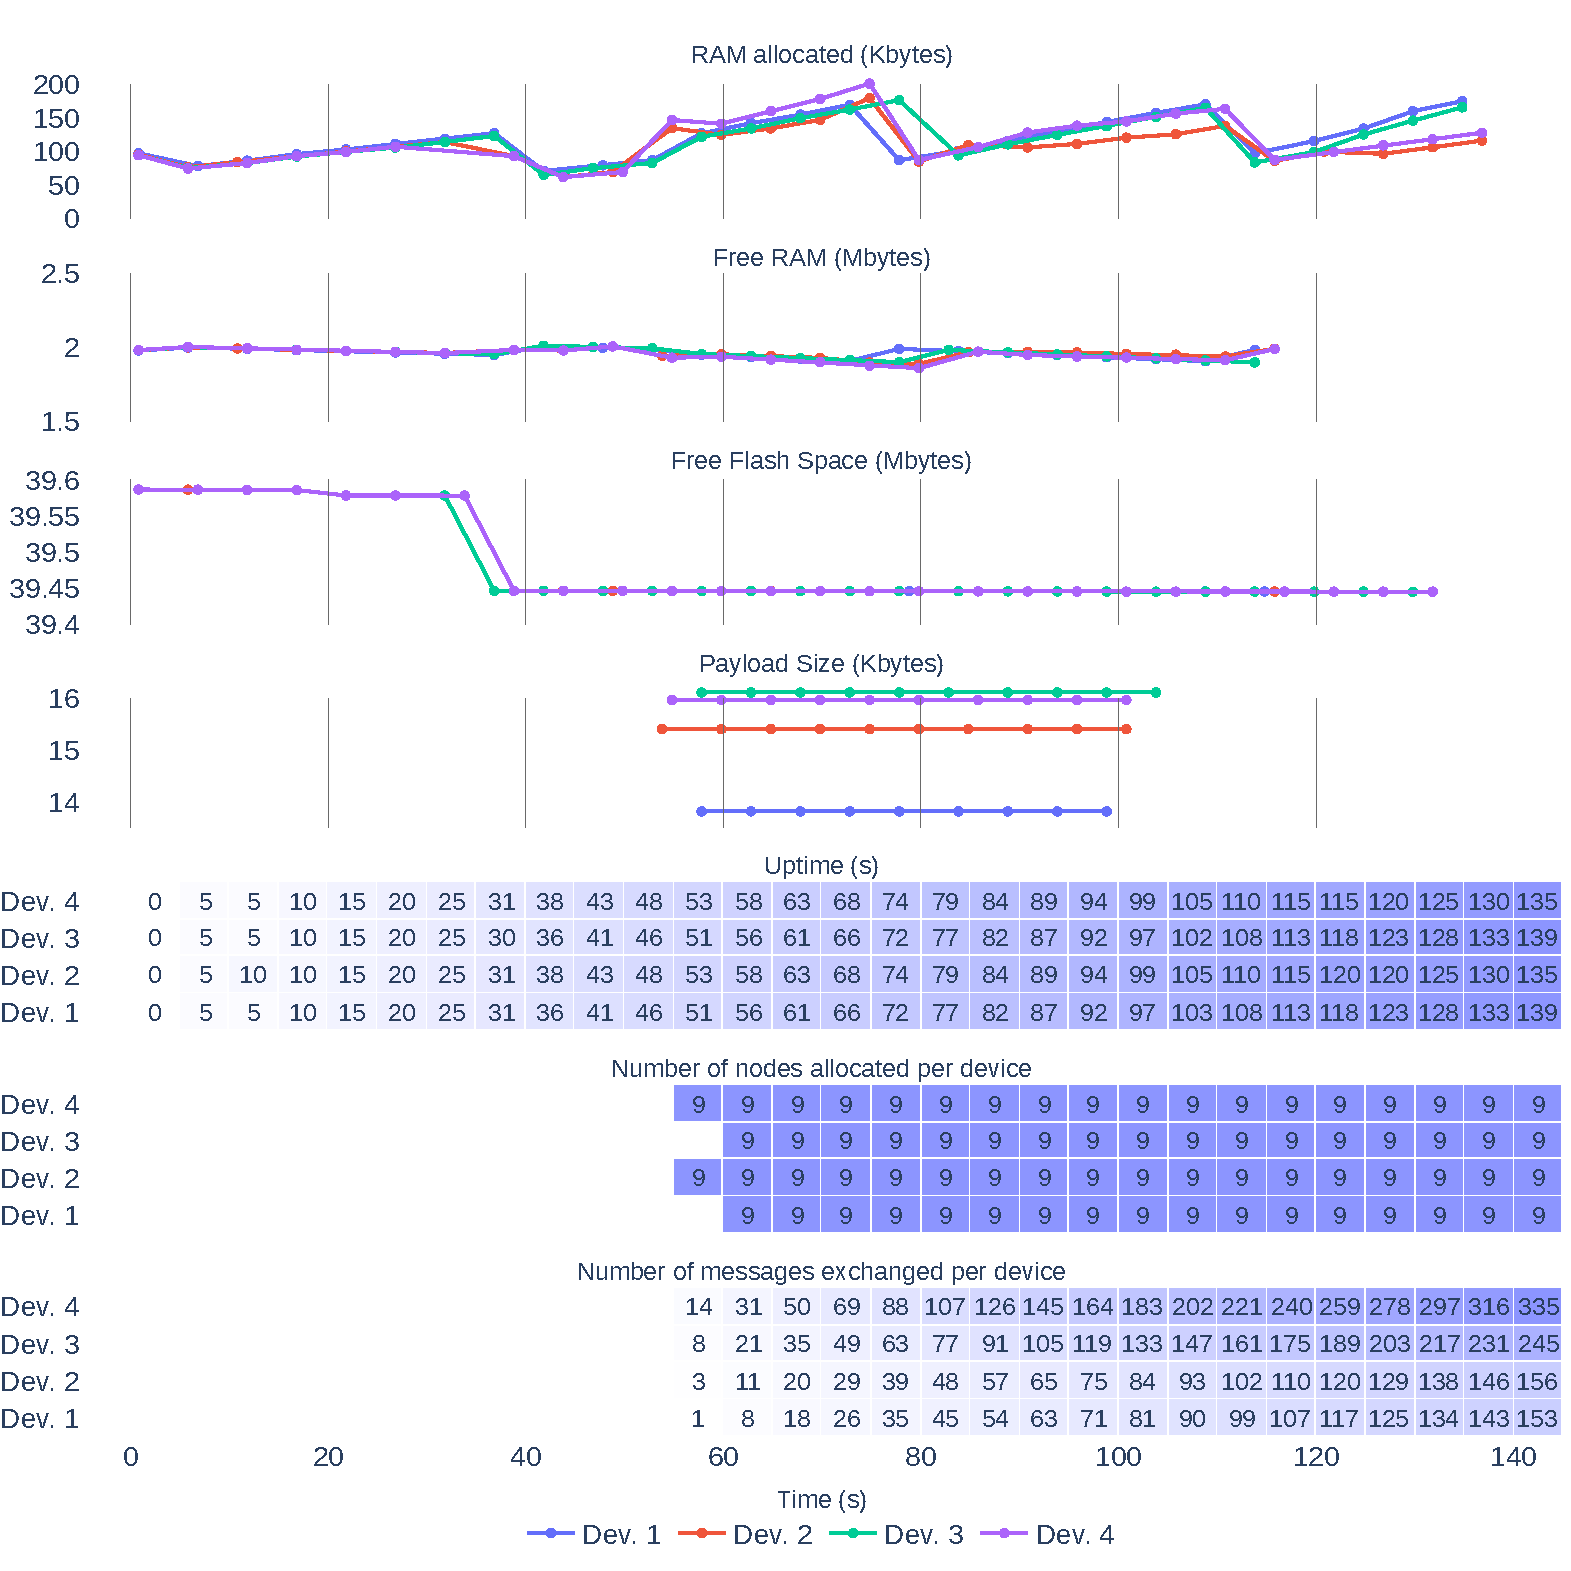
\includegraphics[width=\linewidth]{experiences/1-sanity_check/sanity_check.pdf}
\caption[ES1-SC1 measurements.]{ES1-SC1 measurements.}\label{fig:sanity_check_graph}
\end{figure}

\begin{figure}[h]
\centering
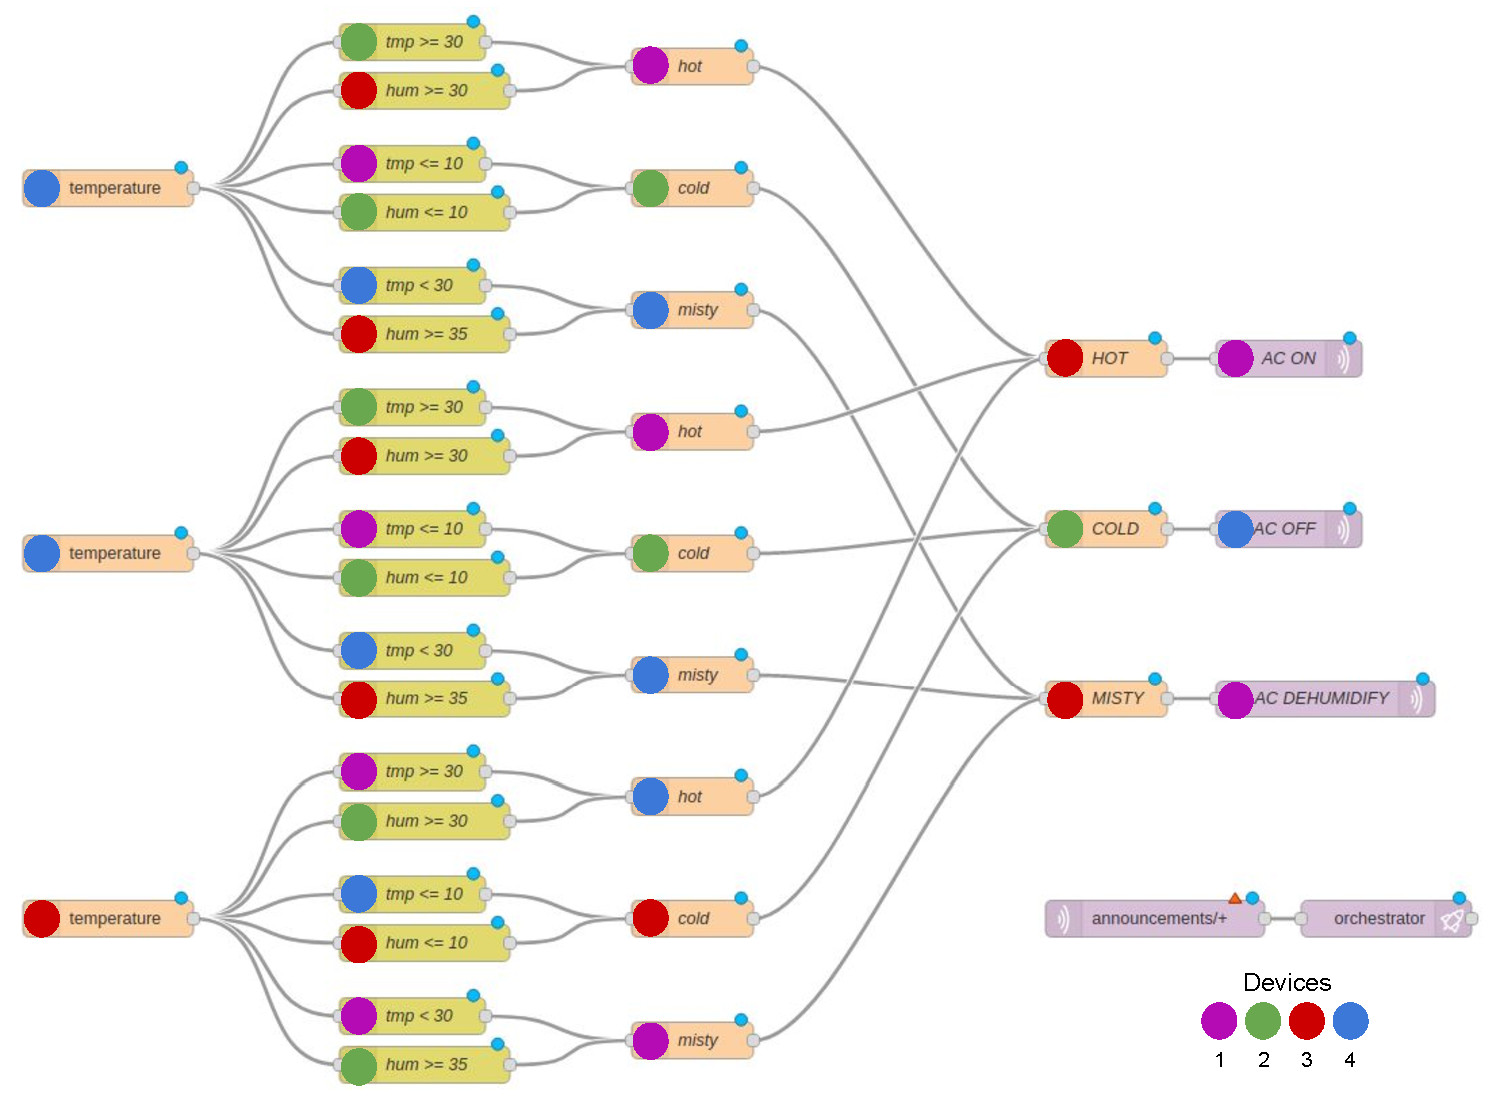
\includegraphics[width=\linewidth]{thesis/figures/experiences/1-sanity_check/node-assignment-visual.pdf}
\caption[ES1-SC1 \textit{node} assignment.]{ES1-SC1 \textit{node} assignment.}\label{fig:sanity_check_node_assignment_visual}
\end{figure}

The usage of RAM was significant, varying from 60Kb to 200Kb \seefigureref{fig:sanity_check_graph}. The flash size only decreases around 150000 bytes, when the device receives a script to execute --- matching the size of the payload received by the devices.

As the orchestrator defines the \textit{nodes} assignment, a script is built and send to the devices. The confirmation of this delivery is necessary for the system to conclude the assignment phase and start monitoring the state of the system.  The time it takes to deliver the script was timed and it can be consulted in \figureref{fig:sanity_check_delivery_time}. The usage of virtual devices running in the same host as the Node-RED instance allows for smaller times, which are measured in milliseconds.

\begin{figure}[h]
\centering
\includegraphics[width=\linewidth]{experiences/1-sanity_check/delivery_time_table.pdf}
\caption[ES1-SC1 script delivery time.]{ES1-SC1 script delivery time.}\label{fig:sanity_check_delivery_time}
\end{figure}

Once the devices execute the script given to them, each \textit{node} allocated to a device start to communicate with each other. To verify that the system works, the messages of all communicating topics were capture, which allowed us to verify that all \textit{nodes} are receiving the messages and producing the expected output messages . The number of communications can be consulted in \figureref{fig:sanity_check_graph}. As it can be observed, the number of messages produced by \textit{Device 4} is bigger than any other. This is due to the fact that in this device two temperature-humidity \textit{nodes} were allocated, which publish 3 messages which are more than the produced by any other device. The \textit{Device 3} contains the other temperature-humidity node \seefigureref{fig:sanity_check_node_assignment_visual}.

To verify if the script delivery time is directly related with the payload size, this experiment was repeated 10 times and the script delivery time for each device was measured. By analyzing \figureref{fig:delivery_times_comp}, we can observe that the script delivery times between devices is very similar. Therefore, there is no relation between payload size and script delivery time. This verification allowed the making of an average of the delivery time, which is $~0.304\pm0.165$s. 

\begin{figure}[h]
\centering
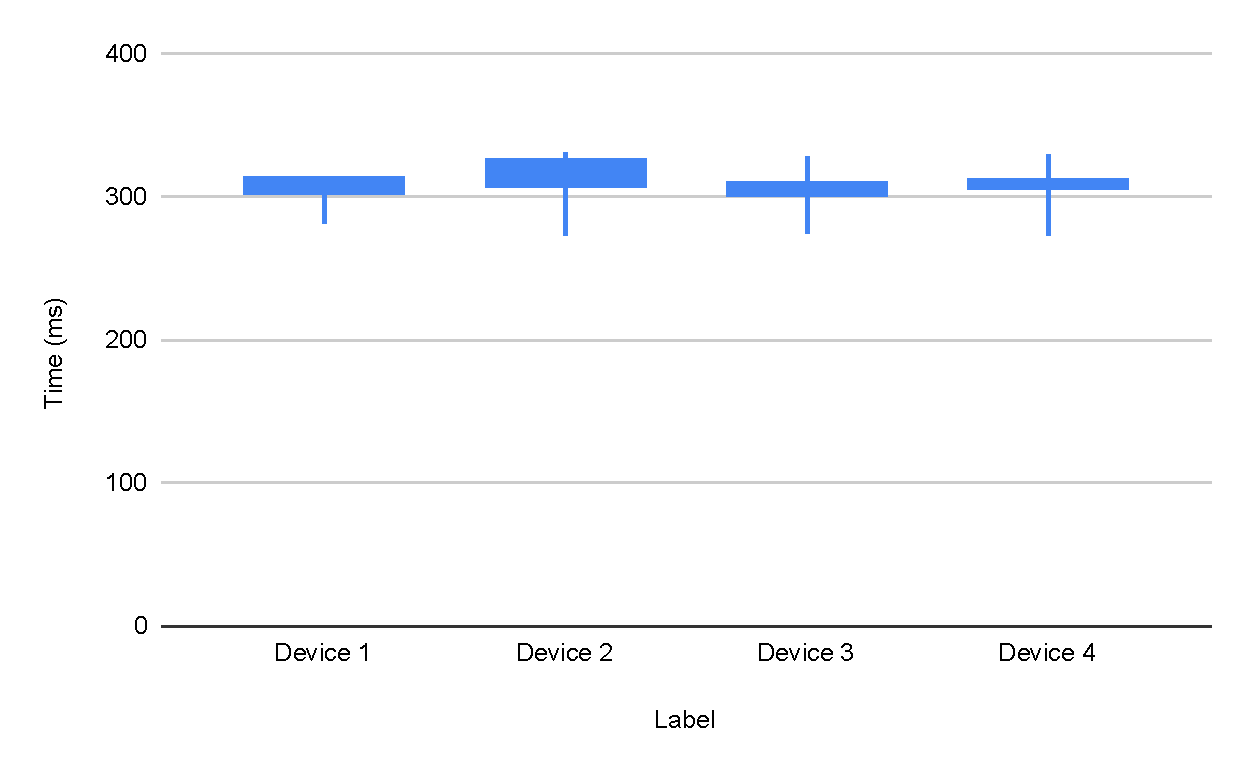
\includegraphics[width=\linewidth]{experiences/1-sanity_check/sending_script_times_comp.pdf}
\caption[ES1-SC1 delivery times.]{ES1-SC1 script delivery times.}\label{fig:delivery_times_comp}
\end{figure}

The sanity check approach performs as expected in a virtual-only setup by (1) spreading the computation amongst available resources and (2) maintaining the system within expected behaviour.

%%%%%%%%%%%%%%%%%%%%%% SC Phys %%%%%%%%%%%%%%%%%%%%%%

\subsubsection{ES1-SC2}\label{sec:sanity_check_phys_exp}

The sanity check experiment was repeated using physical devices, more specifically 4 ESP32. Similar to the virtual devices, the assignment of \textit{nodes} to devices spread the number of \textit{nodes} equally, with each device running 9 \textit{nodes} \seefigureref{fig:sanity_check_phys_graph}.

\begin{figure}[h]
\centering
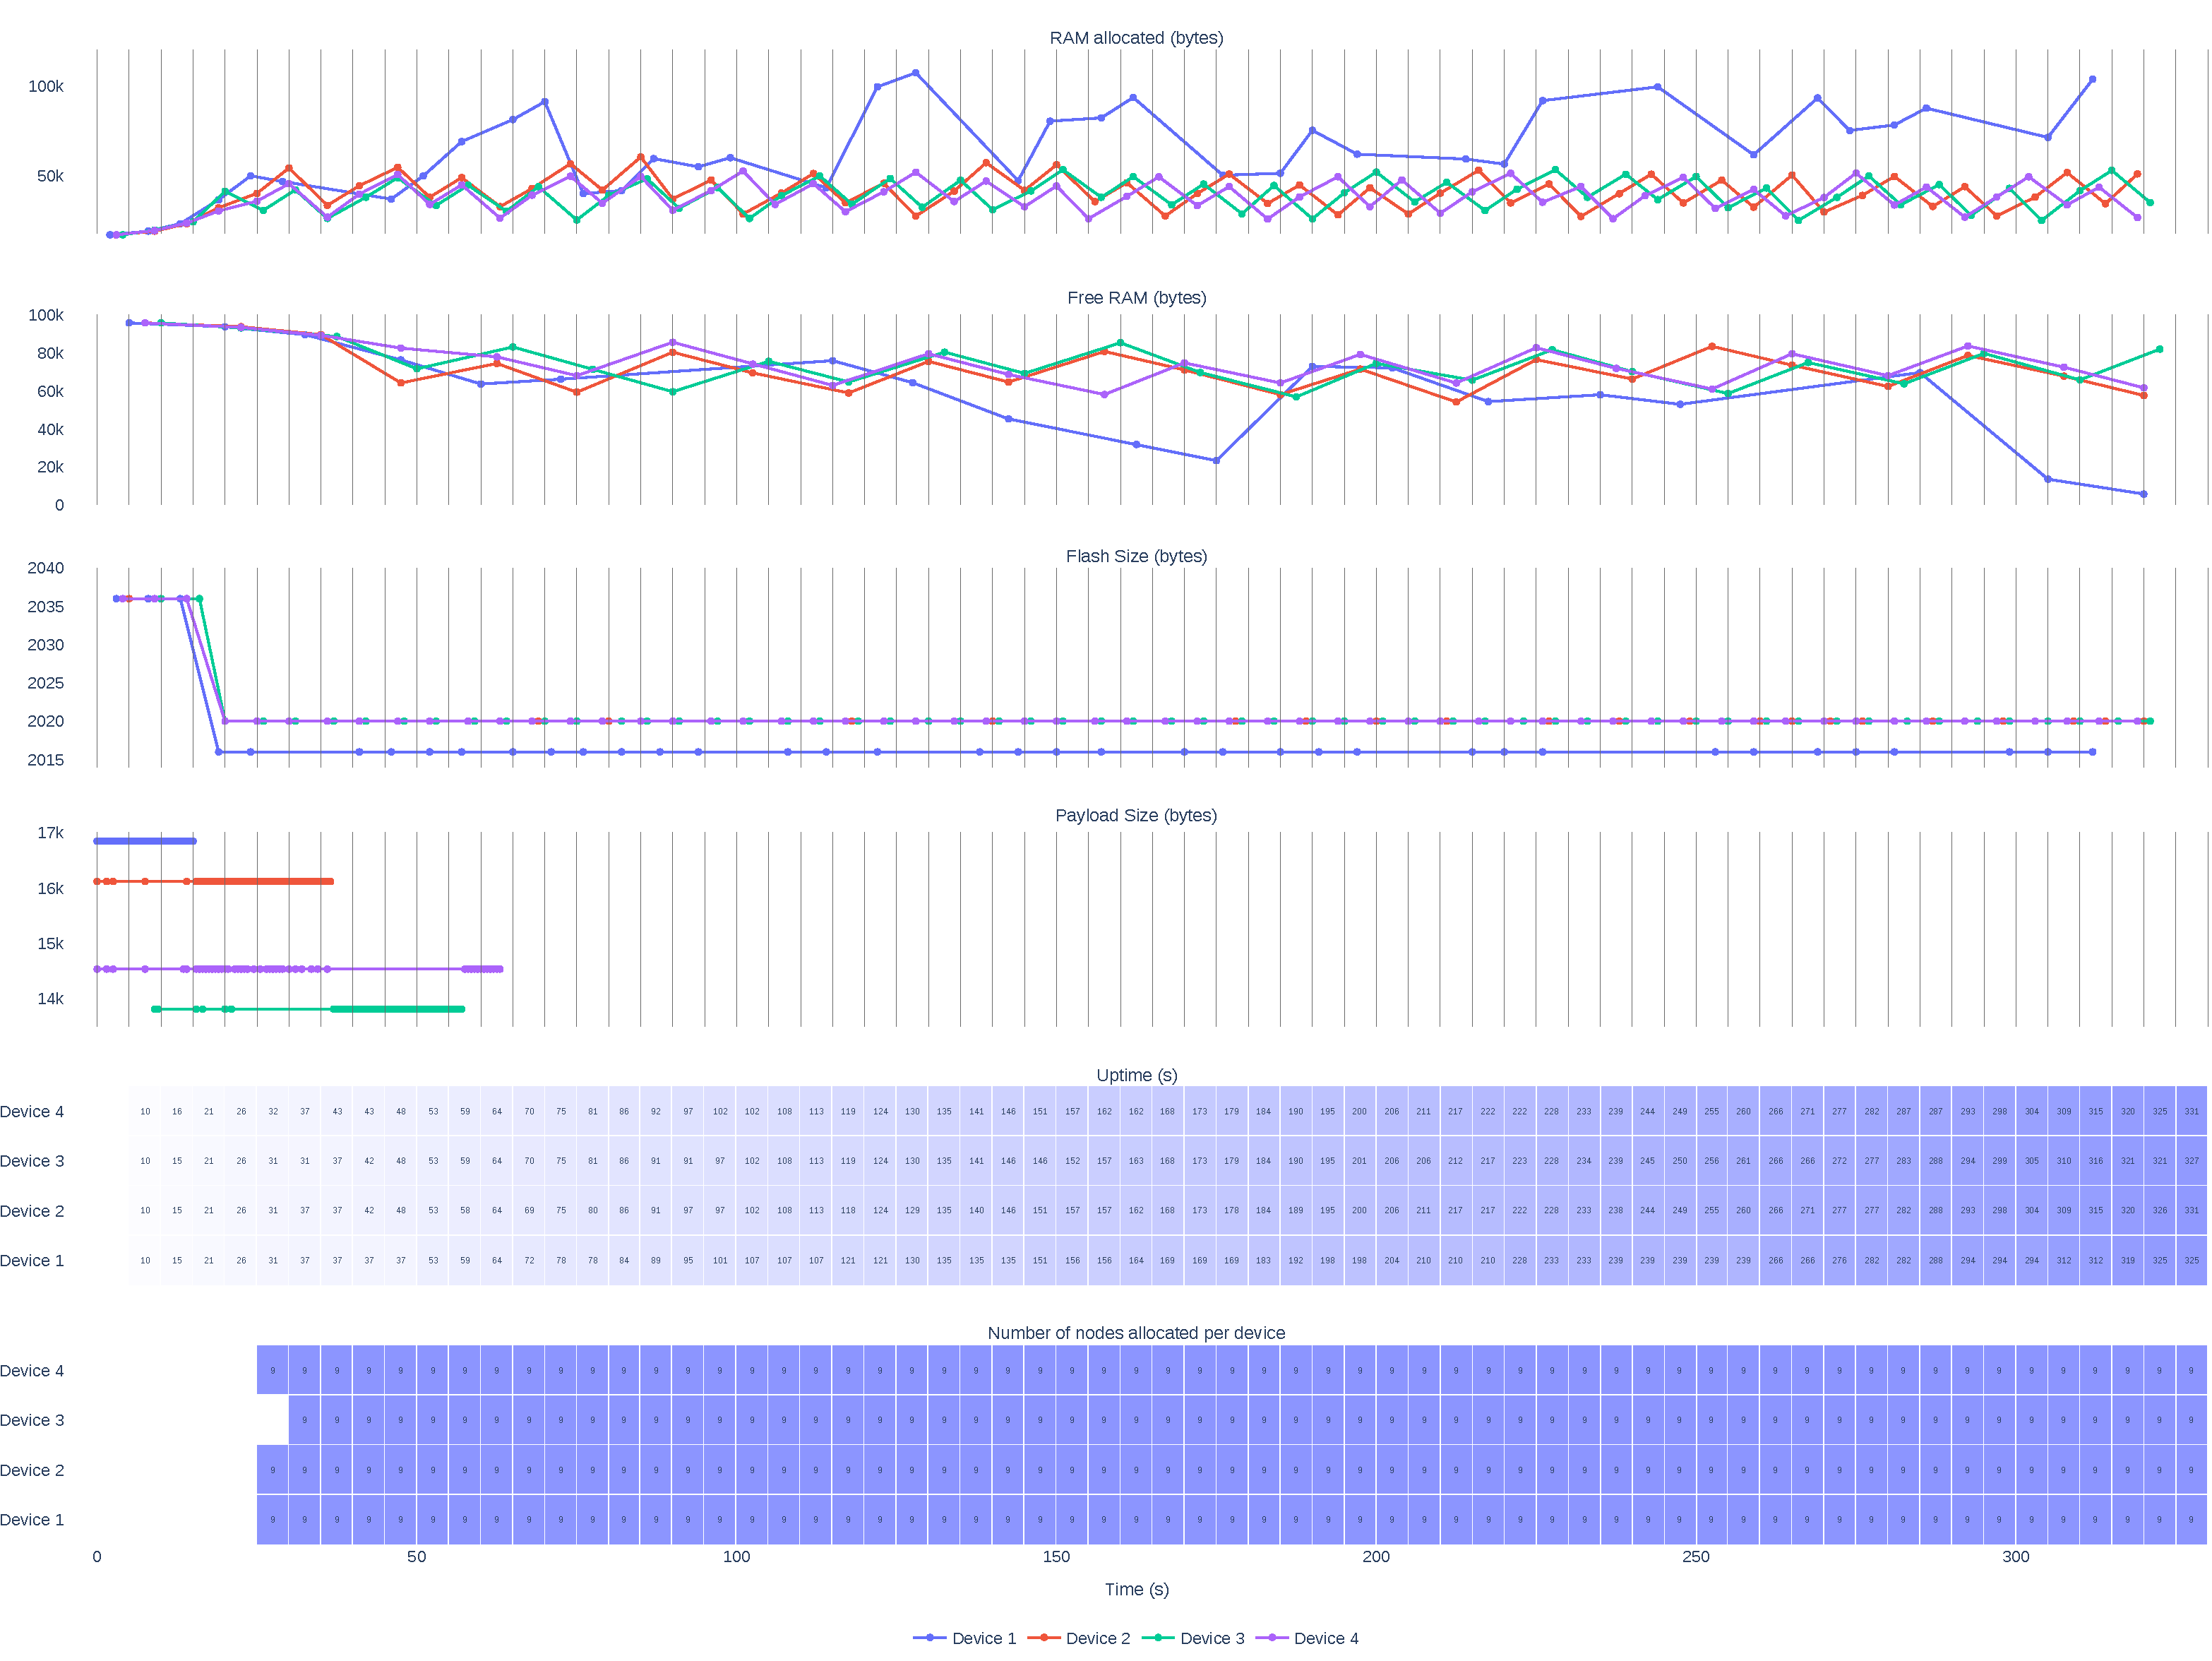
\includegraphics[width=\linewidth]{experiences/1-sanity_check_phys/sanity_check_hardware.pdf}
\caption[ES1-SC2 measurements.]{ES1-SC2 measurements.}\label{fig:sanity_check_phys_graph}
\end{figure}

The usage of RAM in physical devices is smaller than the one used by virtual devices. This can be explained with the possible optimization differences in the Docker-compatible and ESP-compatible MicroPython firmware and libraries.

The free flash space of the physical devices is smaller than the virtual ones, as expected. \figureref{fig:sanity_check_phys_graph} shows that the device with the biggest payload, \textit{Device 1}, ends up having less free flash space. The overall size of the payloads are very similar to the ones in the \textbf{ES1-SC1}. 

\begin{figure}[h]
\centering
\includegraphics[width=\linewidth]{experiences/1-sanity_check_phys/delivery_time_table.pdf}
\caption[ES1-SC2 script delivery time.]{ES1-SC2 script delivery time.}\label{fig:sanity_check_phys_delivery_time}
\end{figure}

The script delivery time for physical devices is bigger than their virtual counterpart, with an average of $~6.578\pm0.476$s \seefigureref{fig:sanity_check_phys_delivery_time}. Since things are not running in the same machine, the Wi-Fi stack and the devices' hardware  characteristics hinder the communication speed. The uptime is similar to the previous experiment, since there were no hardware failures.

%%%%%%%%%%%%%%%%%%%%%% Exp A %%%%%%%%%%%%%%%%%%%%%%

\subsection{ES1: Experimental Tasks}\label{sec:discussion_scenario1_exp}

These experiments focus one validating and evaluating the tool's capacity to adapt to devices' failures. Since the previous experiments (\cf \seesectionref{sec:discussion_scenario1}) already proved that the system executes the tasks that are given to them, this verification will not be repeated in this section's experiments.

\subsubsection{ES1-A}\label{sec:exp_a}

This experiment evaluates if the system is able to re-orchestrate when a device either fails or (re-)appears (\ie new or recovered). During this experiment, devices were turned off one by one until only one was left running. It is expected that the system detects when a device has become unavailable and re-orchestrates, assigning \textit{nodes} to the available devices. In the end, only one device is running and all the \textit{nodes} are assigned to it.

\begin{figure}[h]
\centering
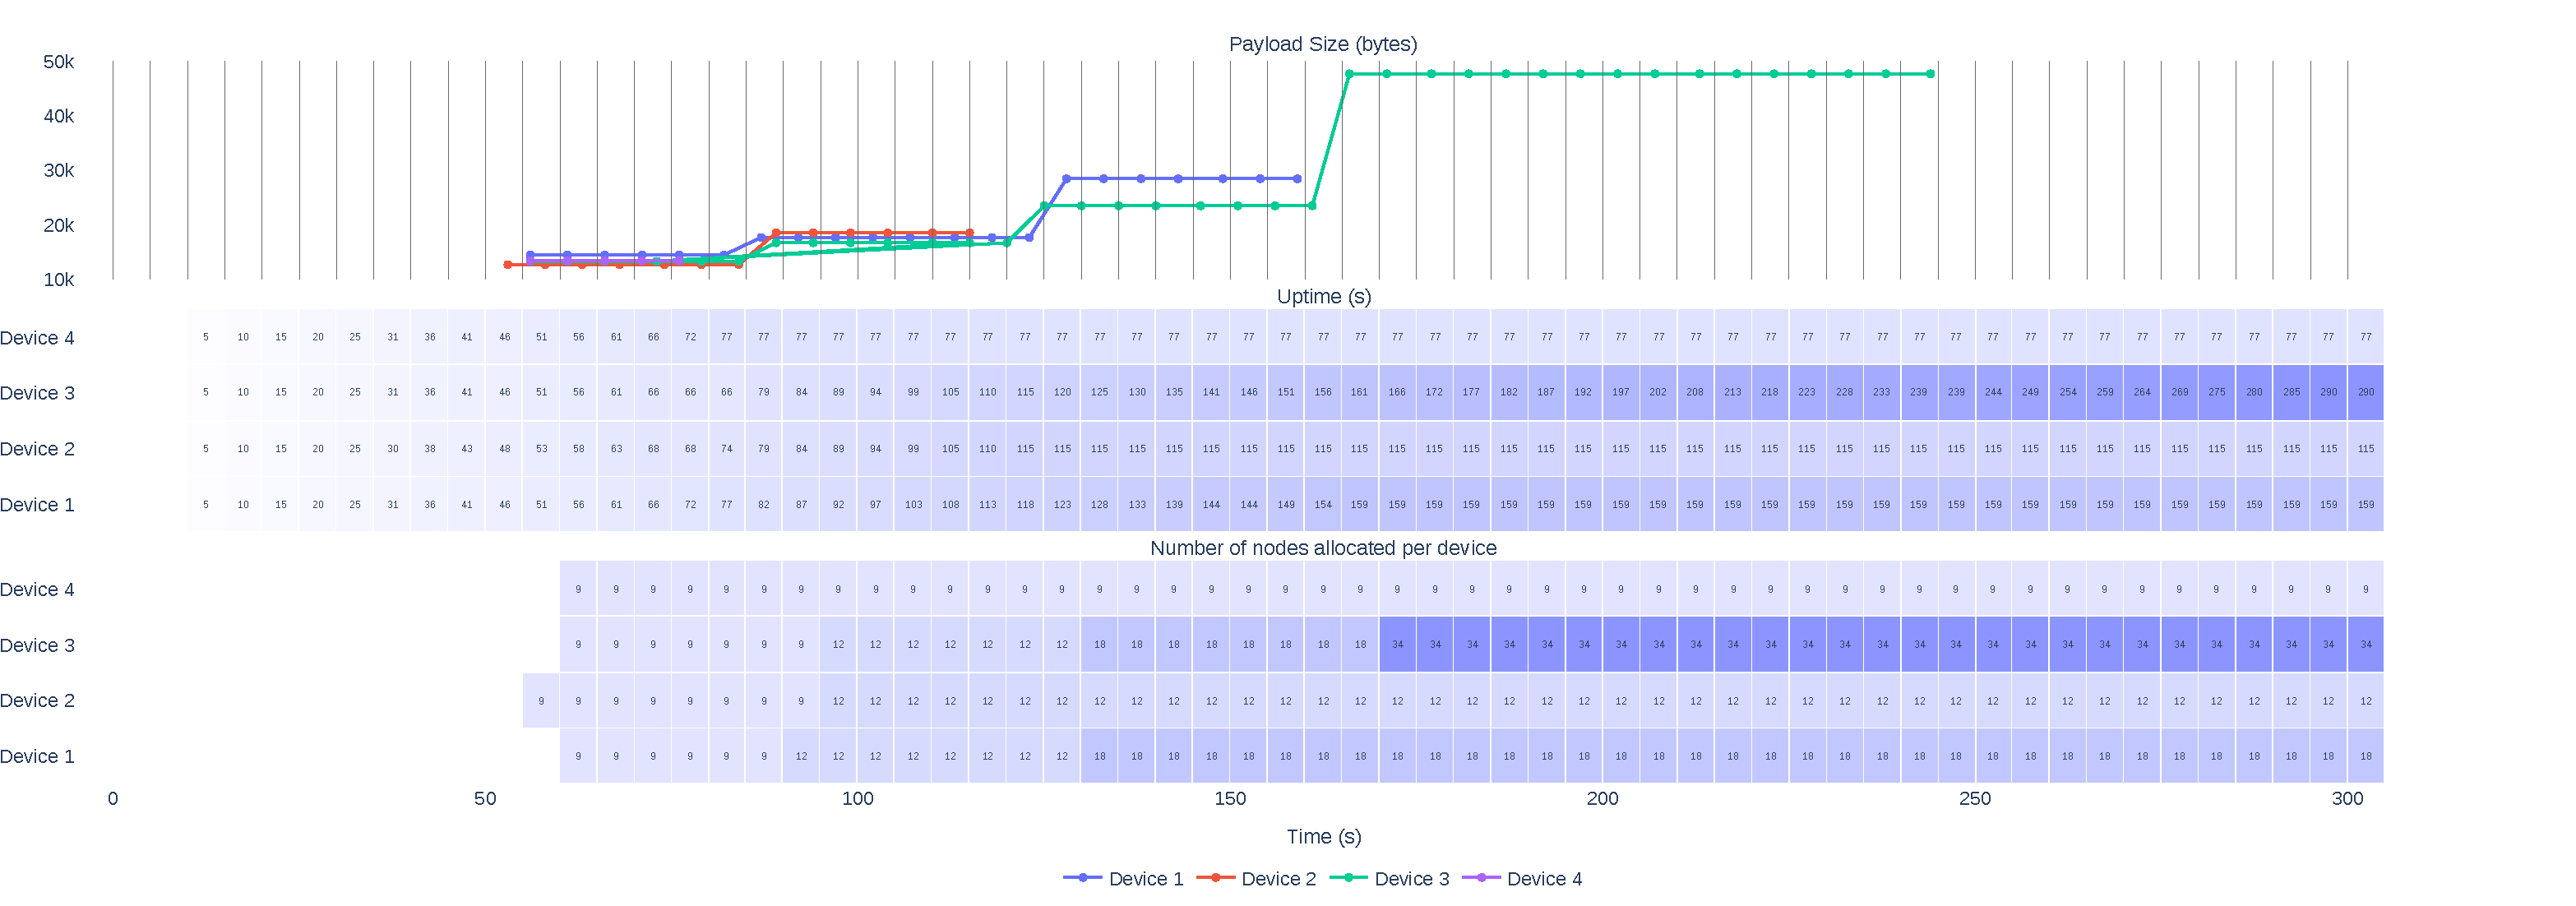
\includegraphics[width=\linewidth]{experiences/A-reorchestration/reorchestration.pdf}
\caption[ES1-A measurements]{ES1-A measurements.}\label{fig:experiment_a_graph}
\end{figure}

\figureref{fig:experiment_a_graph} shows the uptime of the devices stops increasing one by one, identifying the moment the device fails. Once a failure happens, the system re-orchestrates, assigning the \textit{nodes} of the device to the other available devices, increasing their number \seefigureref{fig:experiment_a_graph}. The increase in the number of \textit{nodes} assigned to the available devices can also be observed in the payload size. When all devices fail except one, the one remaining is the only one that receives the payload, which is higher than any other previously received.

The information regarding the number of nodes is not updated to zero once the device fails, since it is no longer active to send the updated metric. 

This allow us to verify that the system identifies the failure of devices and takes actions to rectify it by repeating the assignment process, taking into account the available devices.

%%%%%%%%%%%%%%%%%%%%%% Exp A Phys %%%%%%%%%%%%%%%%%%%%%%

\subsubsection{ES1-B}

Based on \textbf{ES1-A} (\cf \seesectionref{sec:exp_a}), this experiment replaces the virtual devices by physical ones. 

\begin{figure}[h]
    \centering
    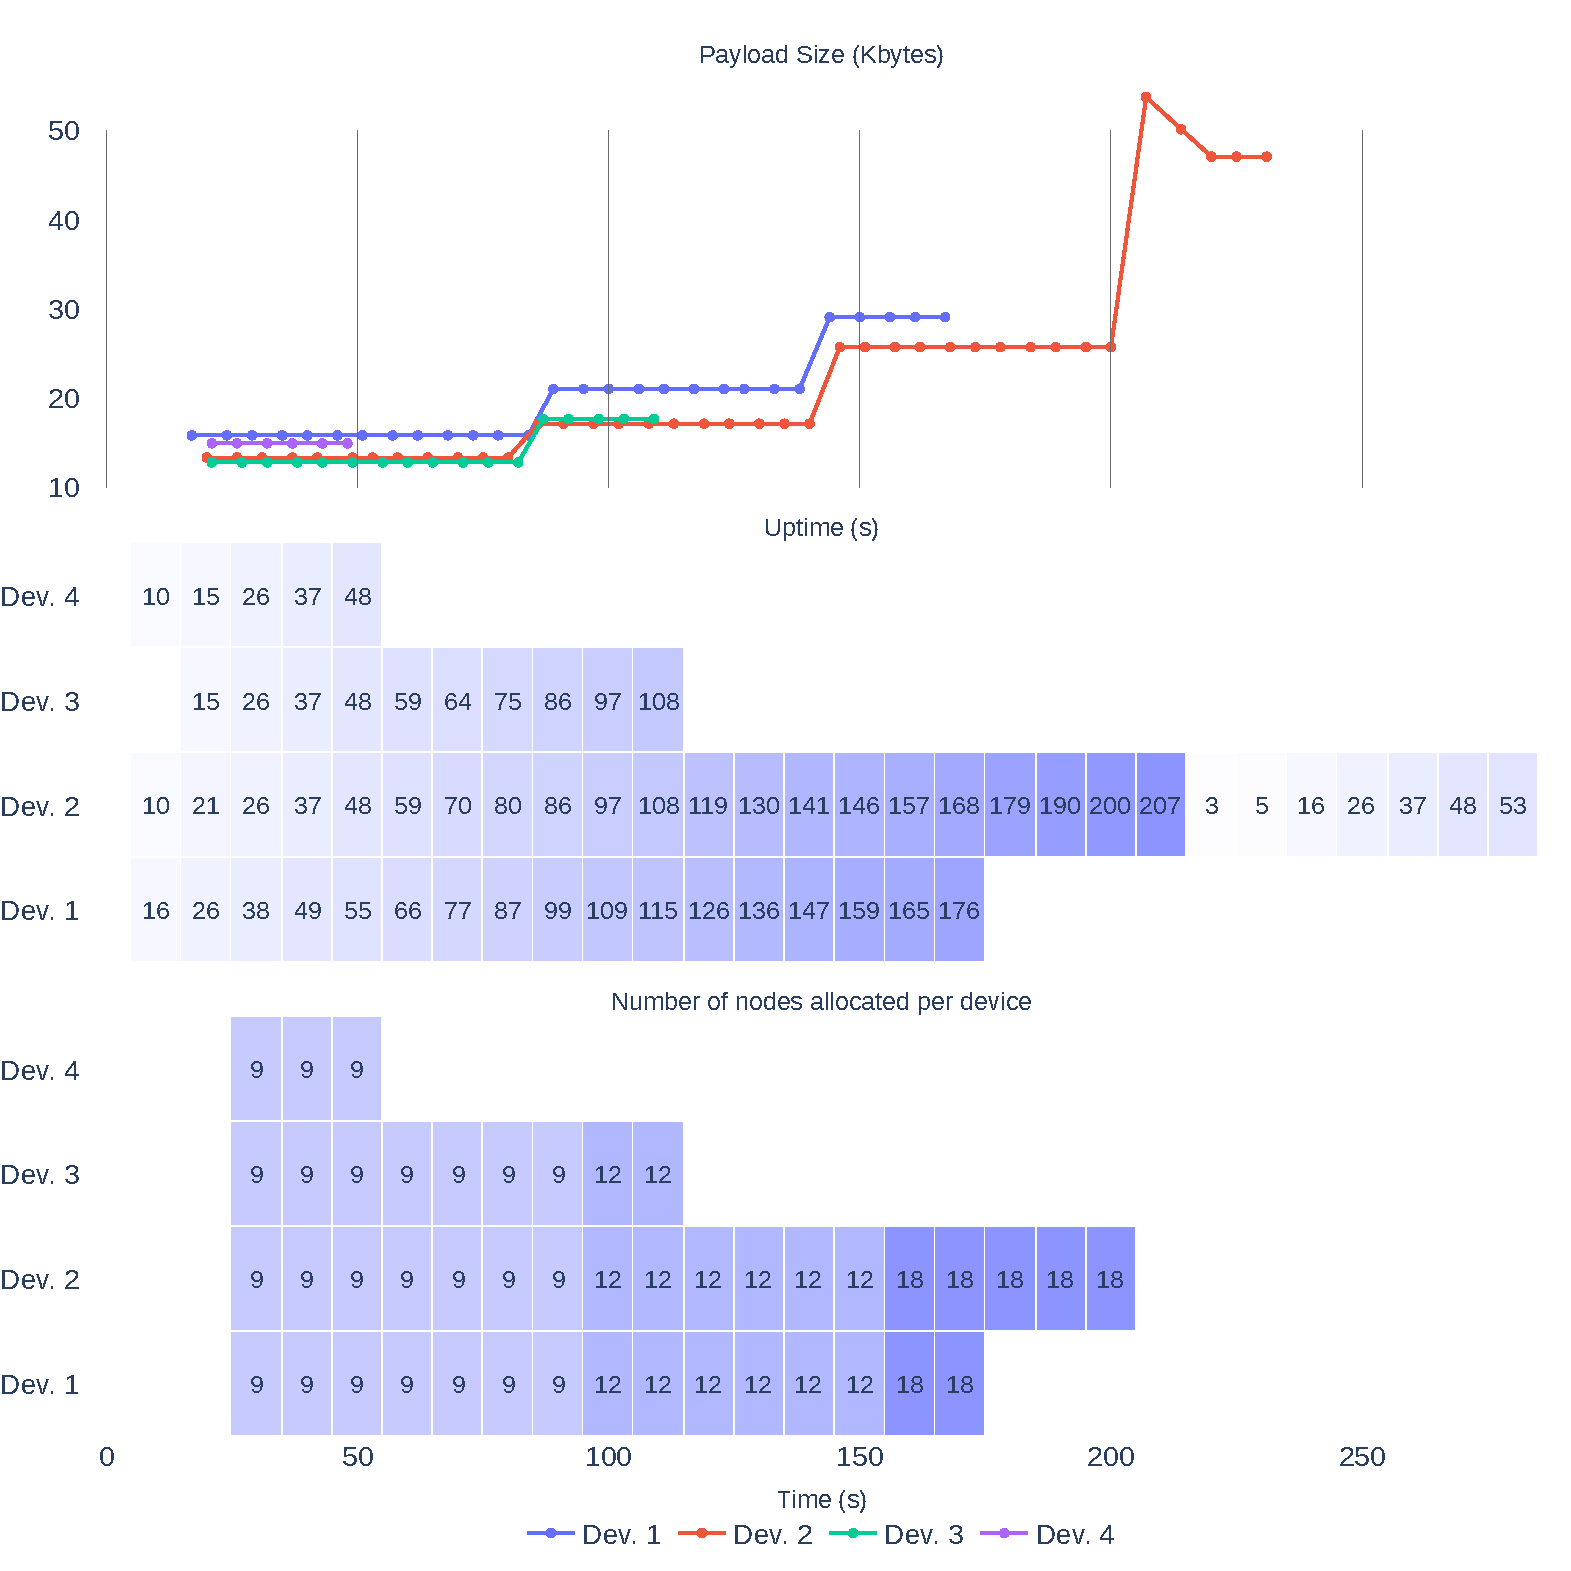
\includegraphics[width=\linewidth]{experiences/A-reorchestration_phys/reorchestration_phys.pdf}
    \caption{ES1-B measurements}
    \label{fig:experiment_a_phys_graph}
\end{figure}

The payloads and number of nodes assigned through the experiment are very similar the experiment \textbf{ES1-A} \seefigureref{fig:experiment_a_phys_graph}. However, it is noticeable that \textit{Device 2}, the last remaining active device, fails when receiving the final-step payload --- which contains the code for all the \textit{nodes} of the system, since no other device is available. 

The device constrained memory does not have capacity to handle the payload size, so it \textsc{fail-safe}s, informing the system that there was an \textit{Out-of-Memory} error, which results in \textit{Orchestrator node} assigning less nodes to the device.

%%%%%%%%%%%%%%%%%%%%%% Exp B %%%%%%%%%%%%%%%%%%%%%%

\subsubsection{ES1-C}

\begin{figure}[h]
    \centering
    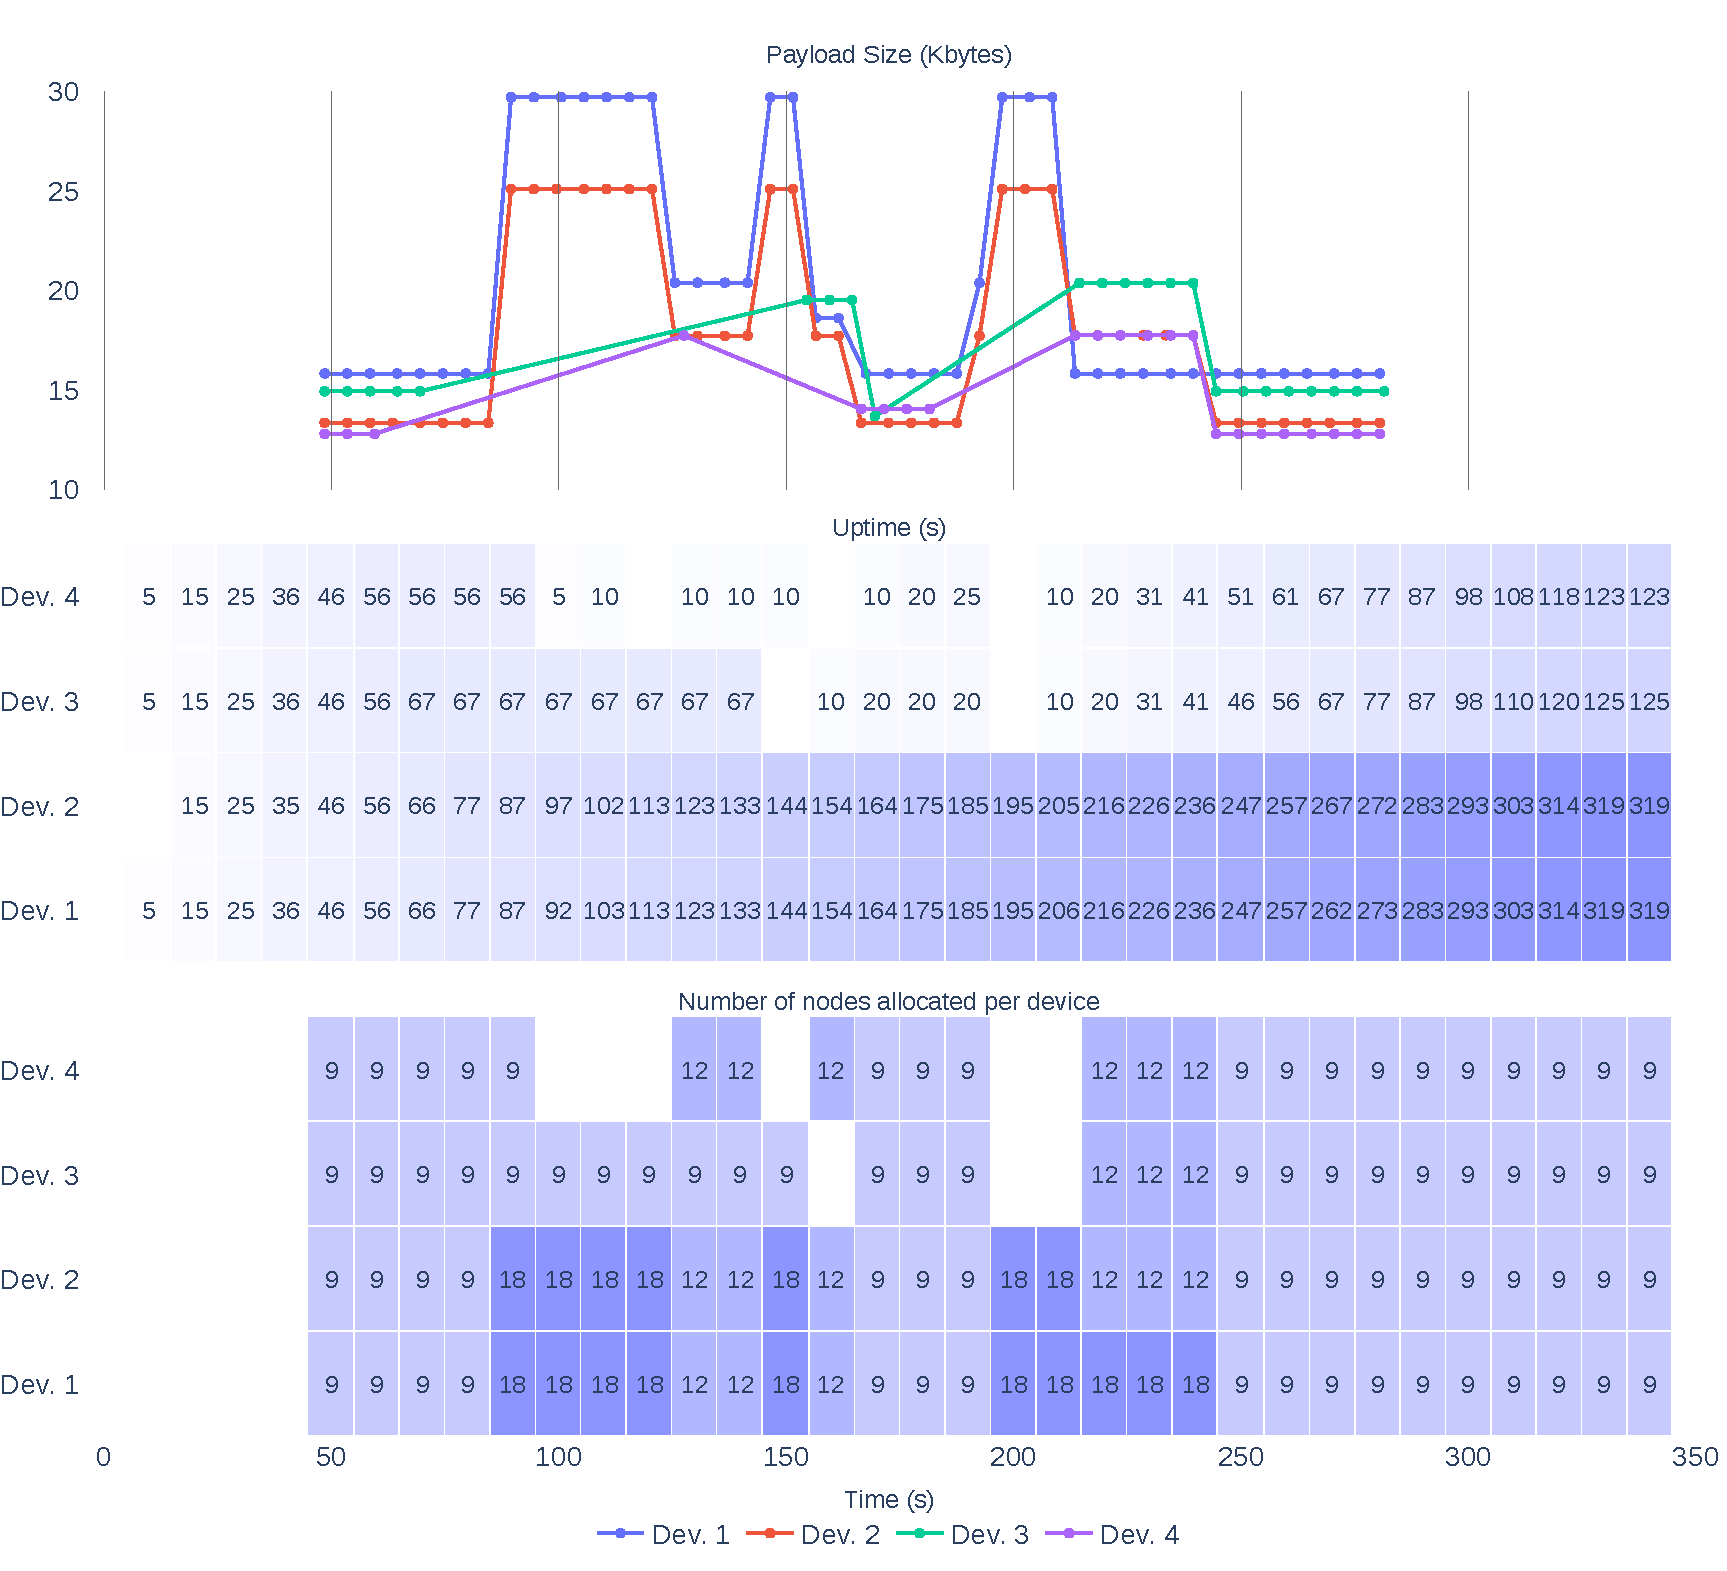
\includegraphics[width=\linewidth]{experiences/B-reorchestration-inconsistent/reorchestration_inc.pdf}
    \caption[ES1-C measurements]{ES1-C measurements.}
    \label{fig:experiment_b_graph}
\end{figure}

Similar to \textbf{ES1-A} and \textit{ES1-B}, this experiment focuses on testing the system's ability to recover when devices fail and then recover. \figureref{fig:experiment_b_graph}, \textit{Device 3} and \textit{Device 4} fail early on and the system recovers, spreading the \textit{nodes} assigned to them to other devices. \textit{Device 4} recovers around the 100s, fails again and then recovers. This change was not caught by the system, since it was very fast, and the system only re-orchestrates the second time \textit{Device 4} recovers. During this experiment \textit{Device 3} and \textit{Device 4} continue to fail and recover, and the system always re-configures itself.

This ability for the system to re-orchestrates when a device recovers can be taxing to the functionality of the system. If a device is constantly failing and recovering, the system will always adapts itself, halting its functionality to orchestrate itself.

%%%%%%%%%%%%%%%%%%%%%% Exp C %%%%%%%%%%%%%%%%%%%%%%

\subsubsection{ES1-D}

This experiment aims to test the system's ability to recover and adapt to the devices' memory constraints. More specifically, memory errors that can arise when writing the received script into the device SPI.

In the \figureref{fig:experiment_c_graph}, both the \textit{Device 2} and \textit{4} are memory constrained. When the first assignment is made, around the 50 seconds, both these devices \textsc{fail-safe} due to \textit{Out-of-Memory} errors. The number of nodes presented in Fig.~\ref{fig:experiment_c_graph} are the ones assigned after devices 2 and 4 communicate to the orchestrator their limitations. 

To assess if the system saves information about the limitations of the devices, one of them was turned of and later turned on. This event is identified in the \figureref{fig:experiment_c_graph}. As it can be observed, \textit{Device 2} uptime stops increasing around the time of the event and its nodes are distributed by the other devices, with the exception of \textit{Device 4}, which is memory constrained. 
After the recovery of \textit{Device 2}, the system (re)orchestrates and the same number of \textit{nodes} is assigned to the devices. However, \textit{Device 4} failed when Device 2 recovered. This implies that the system repeated the process assignment process again, ignoring the previously known information about memory constraints.

\begin{figure}[h]
\centering
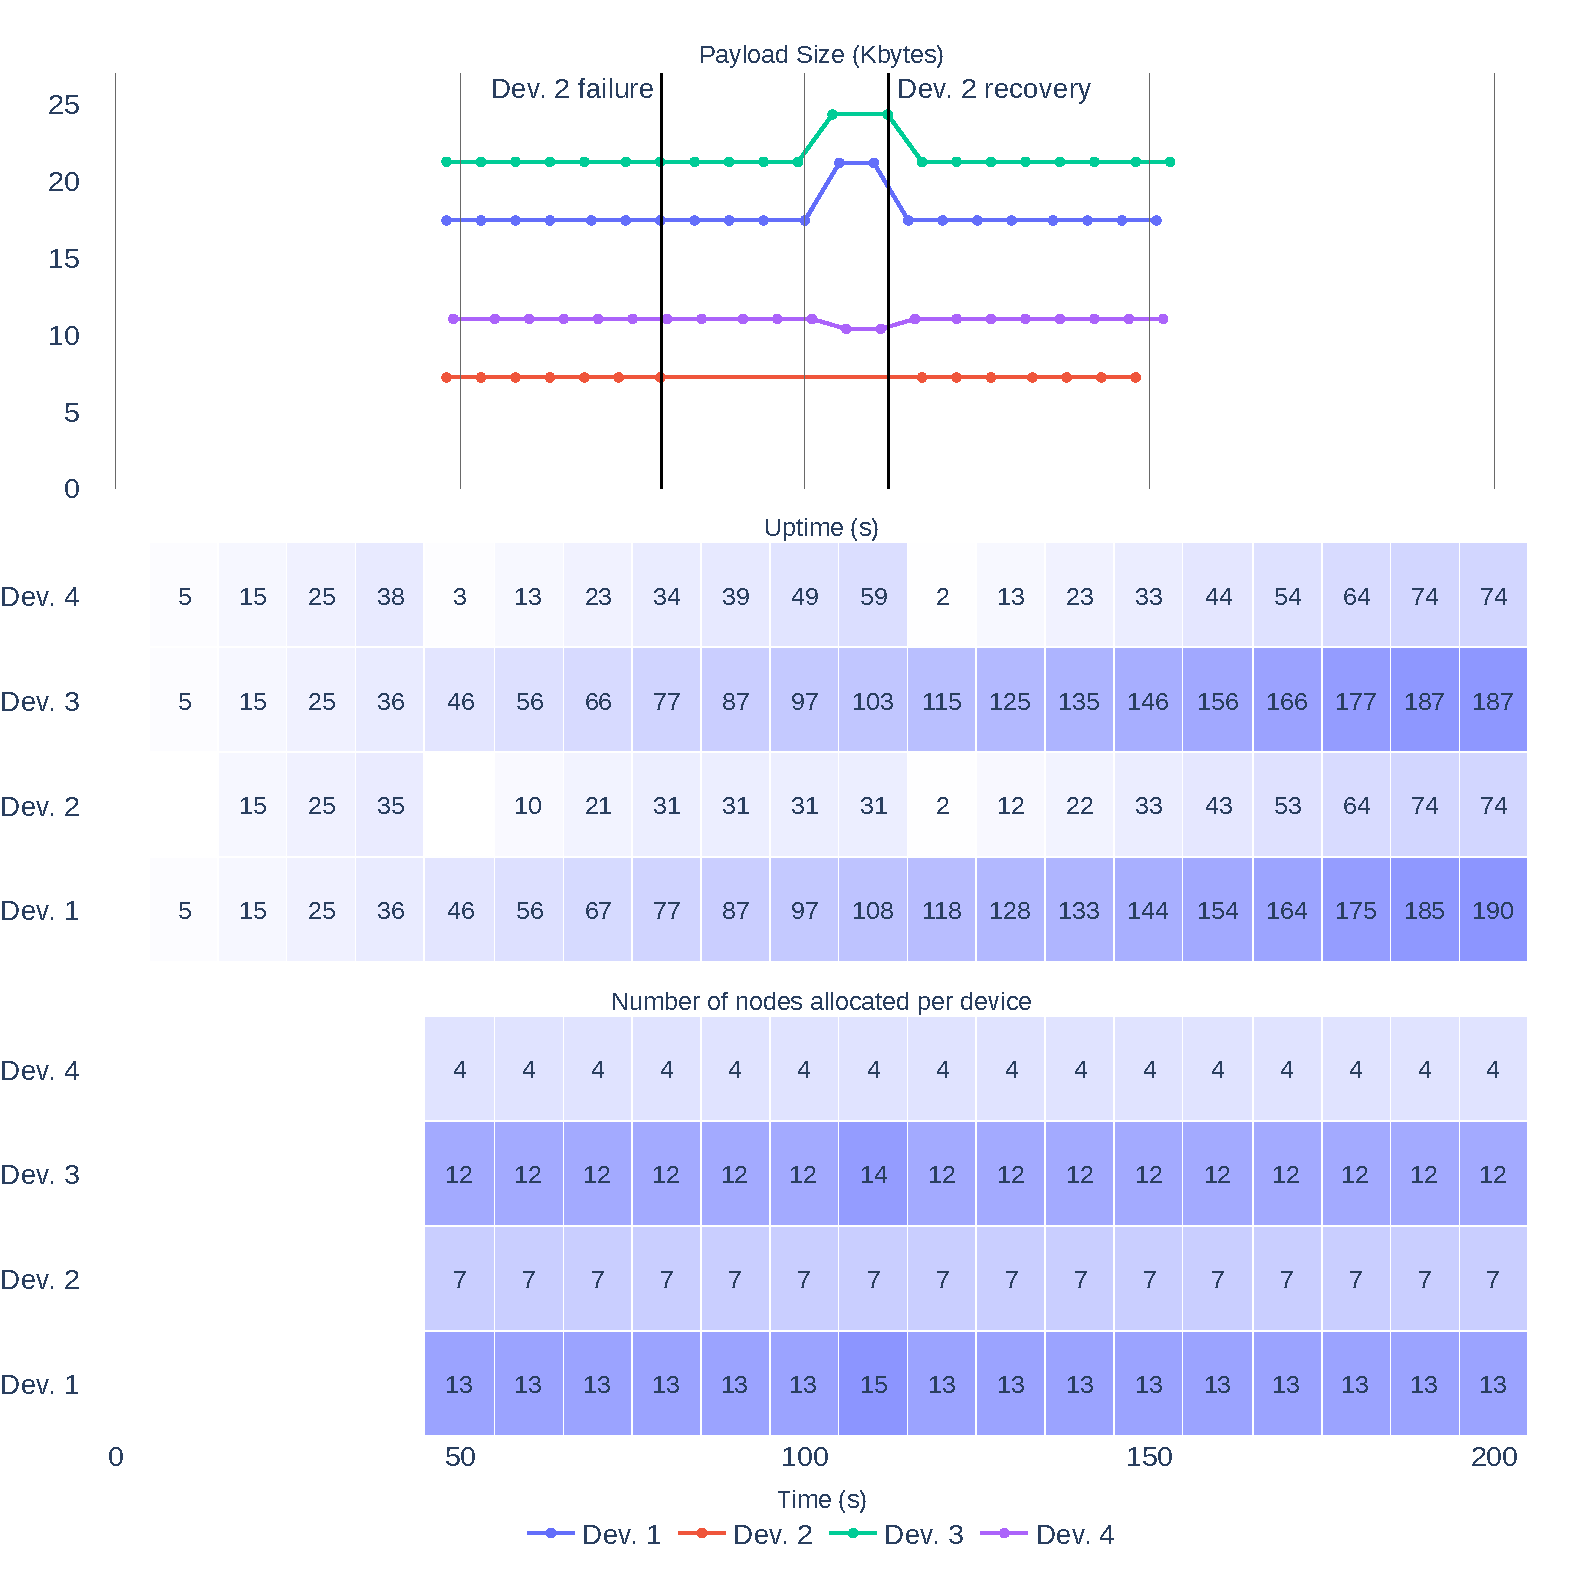
\includegraphics[width=\linewidth]{experiences/C-memory_error_on_write/memory_write.pdf}
\caption[ES1-C measurements]{ES1-C measurements.}\label{fig:experiment_c_graph}
\end{figure}


%%%%%%%%%%%%%%%%%%%%%% Exp D %%%%%%%%%%%%%%%%%%%%%%

\subsubsection{ES1-E}

In this experiment the goal is to check into the system's ability to handle a damaged device that has a memory leak. This device, which in this situation is \textit{Device 2}, will always generate an \textit{Out-of-Memory} error after a random period of time. The system should be able to exclude this device during the course of the assignment process.

As it can be observed in \figureref{fig:experiment_d_graph}, \textit{Device 2} is consistently failing after the first assignment of nodes, around 75 seconds. The number of nodes assigned decreases, until no node is assigned and the device is excluded from consideration. This is an iterative process, in which the system will decrease the number of \textit{nodes} it assigns to a device if the device communicates an \textit{Out-of-Memory} to the orchestrator. Eventually, if the device does not handle any node, the minimum number of \textit{nodes} the device can handle is 0, excluding the device from the assignment process.

\begin{figure}[h]
\centering
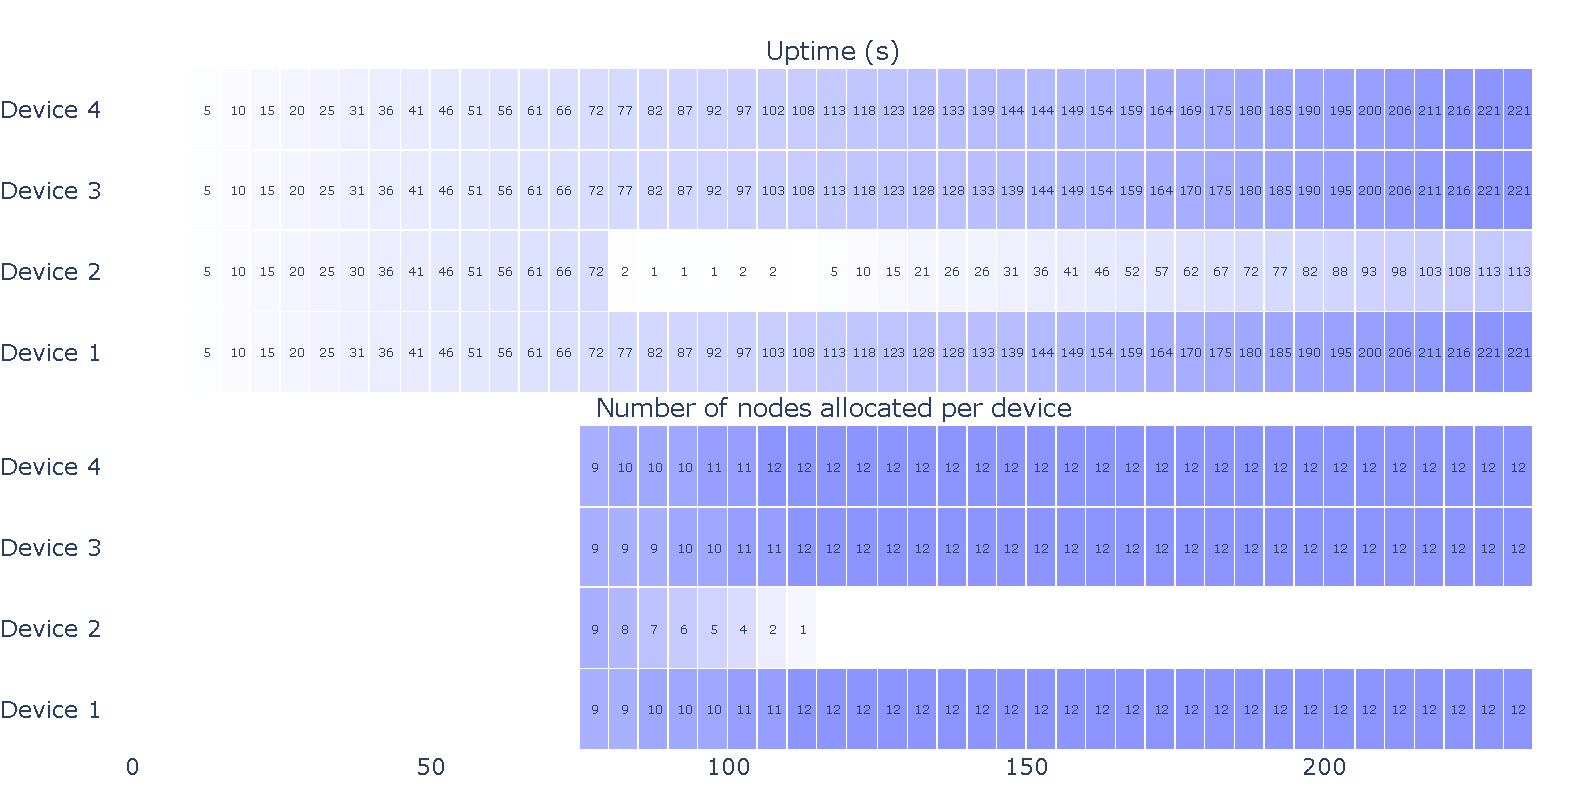
\includegraphics[width=\linewidth]{experiences/D-memory_error_random/memory_random.pdf}
\caption[ES1-E measurements]{ES1-E measurements.}\label{fig:experiment_d_graph}
\end{figure}

%%%%%%%%%%%%%%%%%%%%%% Exp E %%%%%%%%%%%%%%%%%%%%%%

\subsubsection{ES1-F}

This experiment purpose is inject a \textit{node} that causes \textit{Out-of-Memory} errors in specific devices. With this, the system should (re)orchestrate and converge in a solution where the specific \textit{nodes} are assigned to devices not affected by them. In their turn, the devices affected by these \textit{nodes} should have less \textit{nodes} assigned to them. The system and devices do not know that a specific \textit{node} is creating the \textit{Out-of-Memory} errors and interpret the error as a device problem.

Since the first assignment can already be correct by default, meaning that these faulty \textit{nodes} are assigned to devices not affected by them, some changes were made to force the system to (re)orchestrate. The devices were all turned off and on in in different order, this repeated 3 times. These events can be observed in \figureref{fig:experiment_e_graph} around the 125, 200 and 275 second timestamps. It is important to note that the devices affected by the faulty \textit{nodes} are devices \textit{4} and \textit{2}.

The event we aim to test occurs around 300 seconds, however a limitation is apparent. As it can be seen, \textit{Device 1} is assigned 9 \textit{nodes} and \textit{Device 4} is assigned 10. The uptime of \textit{Device 4} resets in this small time period, meaning that an \textit{Out-of-Memory} occurred and the device performed a \textsc{fail-safe}. The system updates, spreading the 10 \textit{nodes} previously assigned to \textit{Device 4} through all the available devices. 

When the system receives information that \textit{Device 4} is available again, it already knows that it has a limitation, so it only assigns 9 \textit{nodes} to it. It can be seen that missing \textit{node} is assigned to \textit{Device 1}. Since \textit{Device 4} does not \textsc{fail-safe}, the \textit{node} assigned to \textit{Device 1} must have been the faulty one.

\begin{figure}[h]
\centering
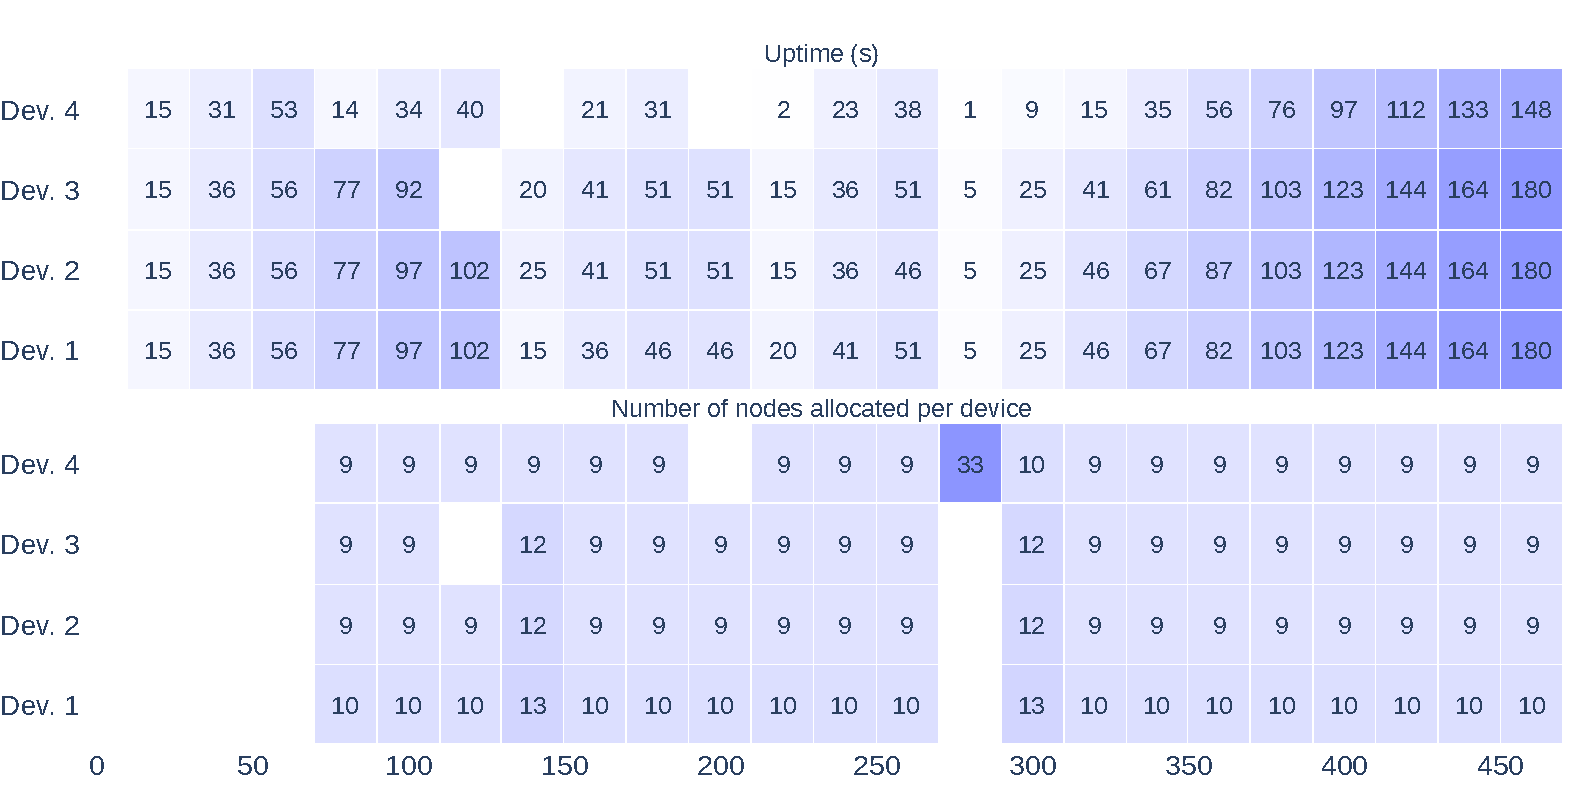
\includegraphics[width=\linewidth]{experiences/E-memory_error_node_failure/memory_failure.pdf}
\caption[ES1-F measurements]{ES1-F measurements.}\label{fig:experiment_e_graph}
\end{figure}

%%%%%%%%%%%%%%%%%%%%%% Exp F %%%%%%%%%%%%%%%%%%%%%%

\subsubsection{ES1-G}\label{sec:experiment_f}

This experiment consists of pushing the system to its limits by introducing constant failures in its devices. Every second, each device has a 5\% probability of becoming unavailable from 0 to 10 seconds. During this period, the device is unresponsive to the orchestrator requests and, when recovered, announces itself.

The results of the experiment can be consulted in Figures \ref{fig:stress_test_nodes} and \ref{fig:stress_test_status}. From \figureref{fig:stress_test_nodes} it can be concluded that the system is constantly (re)orchestrating itself, and once the majority of devices failed, the system becomes unstable. It is important to note that, similar to previous devices, once a device fails, the number of nodes does not update to 0. With this in mind, it can be concluded that devices with the same number of nodes during the total execution of the system failed early on and continued to fail, not allowing another assignment by the orchestrator.

Around the 100 seconds, it can be noted in \figureref{fig:stress_test_status} a period where all devices were available. However, the node assignment in \figureref{fig:stress_test_nodes} does not converge during that time period. The reason for this behaviour is that the system will (re)orchestrate when a device becomes available. Since each device announces itself individually, each announcement triggers a new orchestration. This process takes time and results in several failed orchestrations due to outdated data of the status of the devices. 

This is a limitation of the system, making it vulnerable to a possible DoS attack in the form of an excess of status activity from the devices. This constant orchestration is also taxing for the devices, causing an overload of received assignments that will never make the system function as a whole.

\begin{figure*}[h]
    \centering
    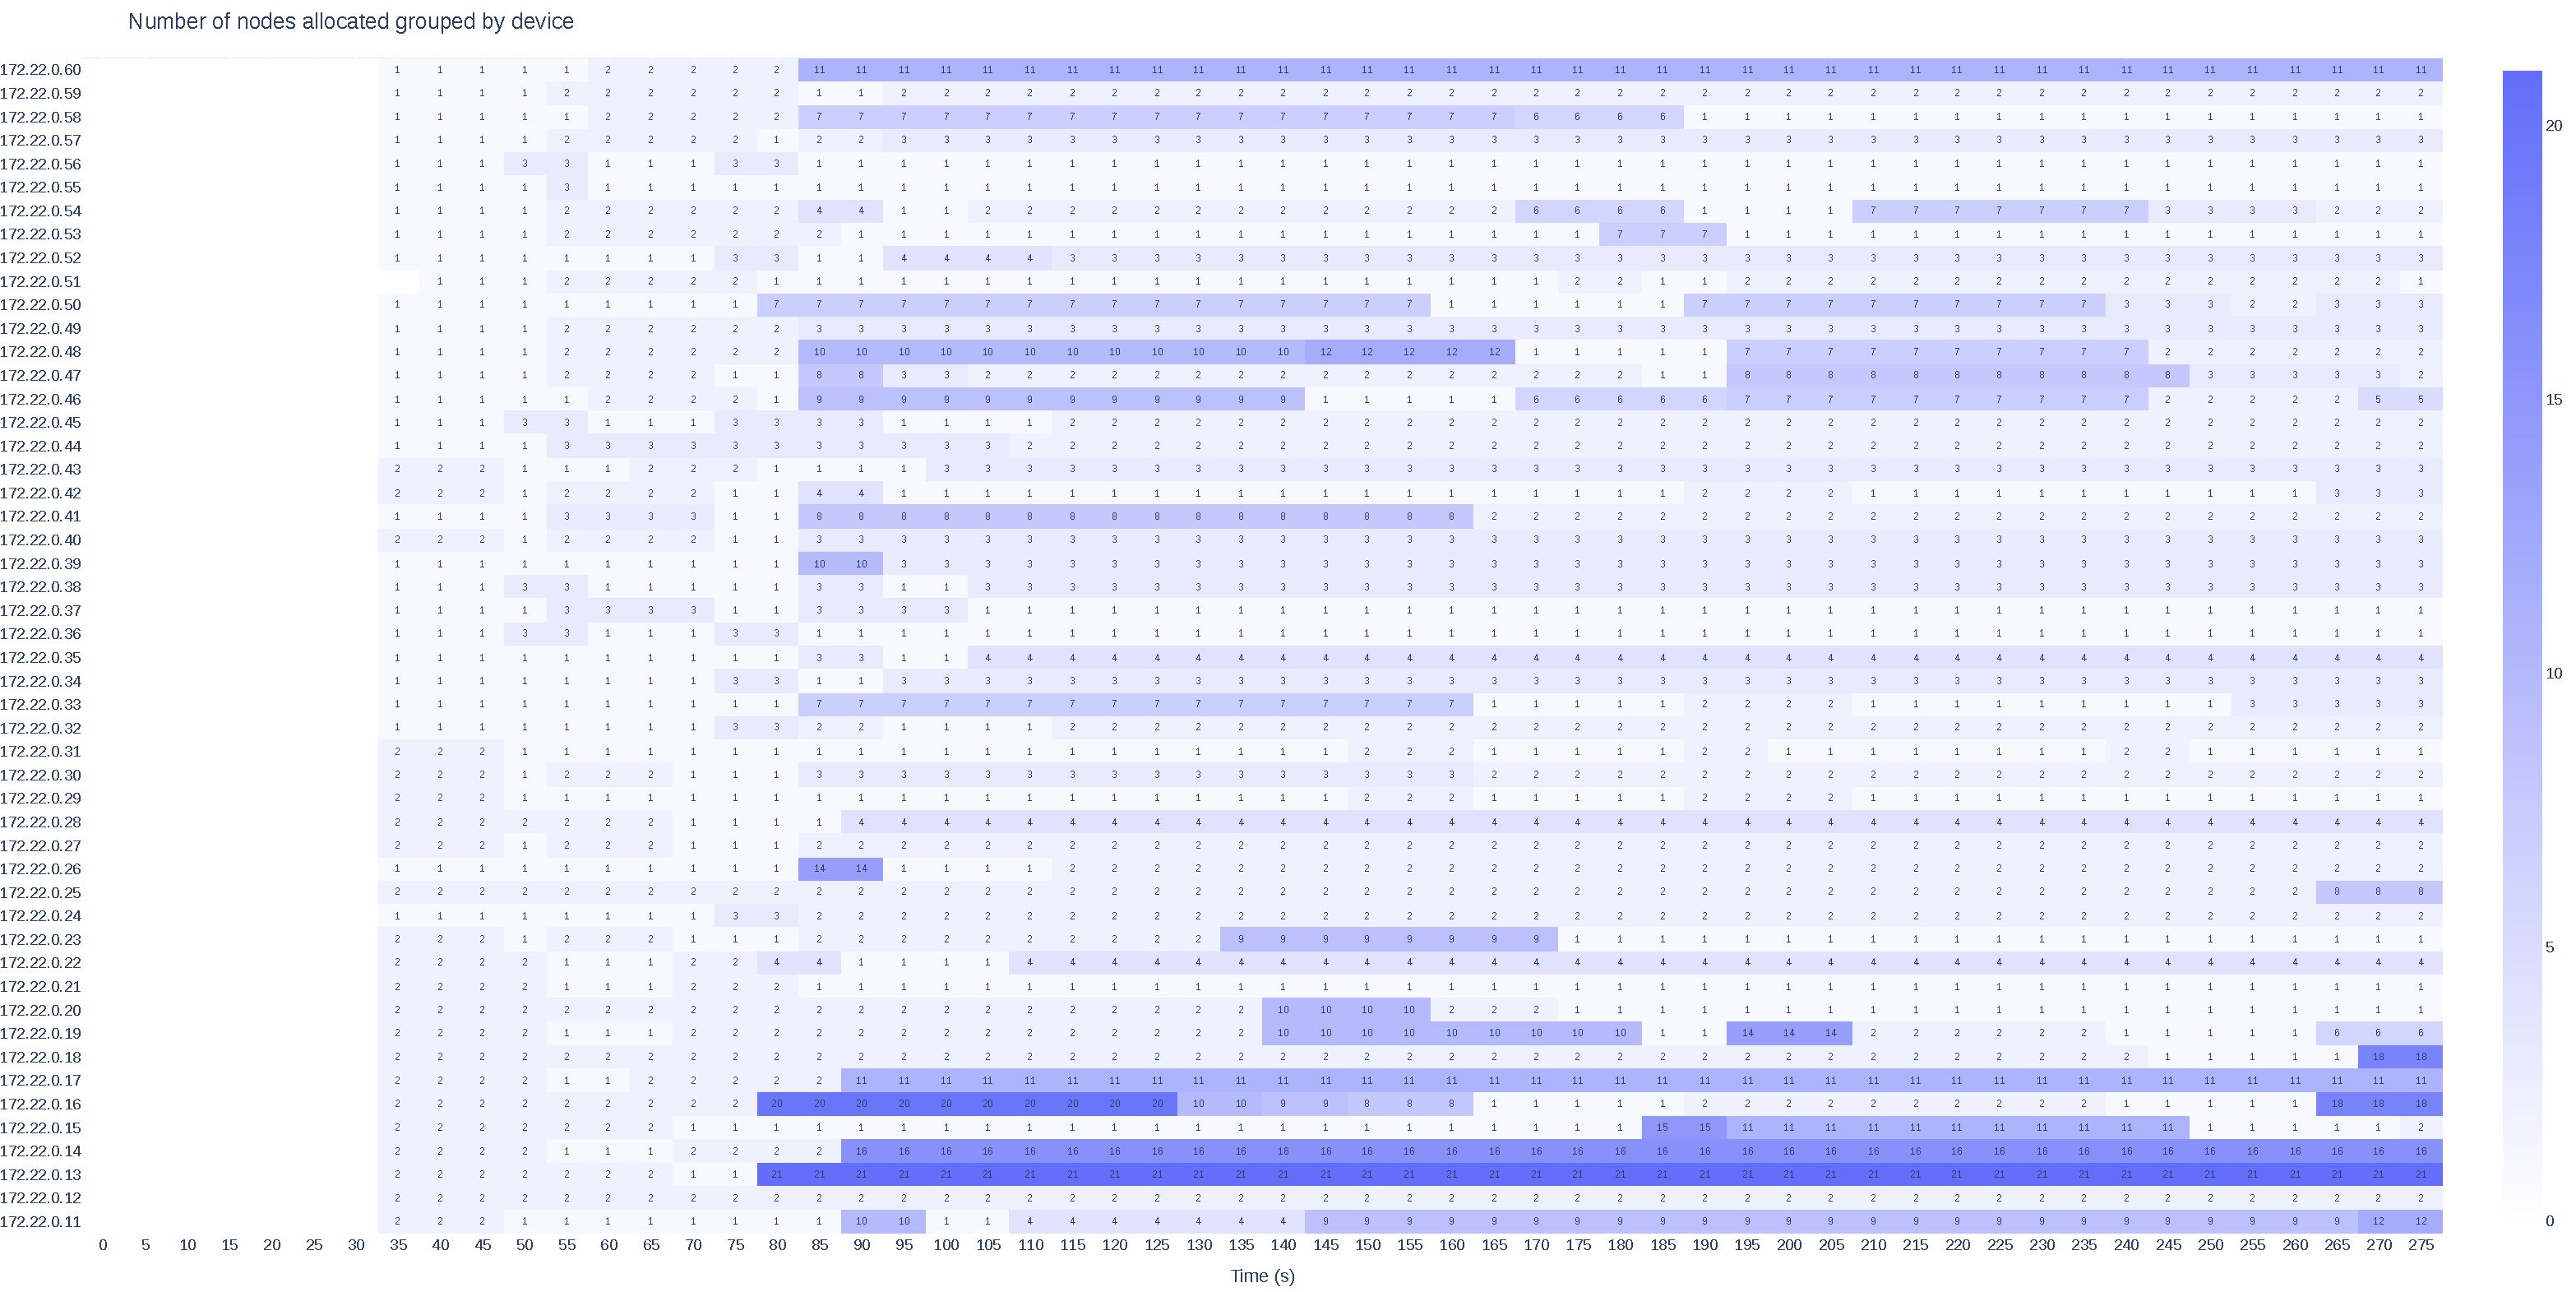
\includegraphics[width=\textwidth]{experiences/F-stress_test/nodes_heatmap.pdf}
    \caption[Nodes assignment distribution]{Nodes assignment distribution}\label{fig:stress_test_nodes}
\end{figure*}

\begin{figure}[h]
\centering
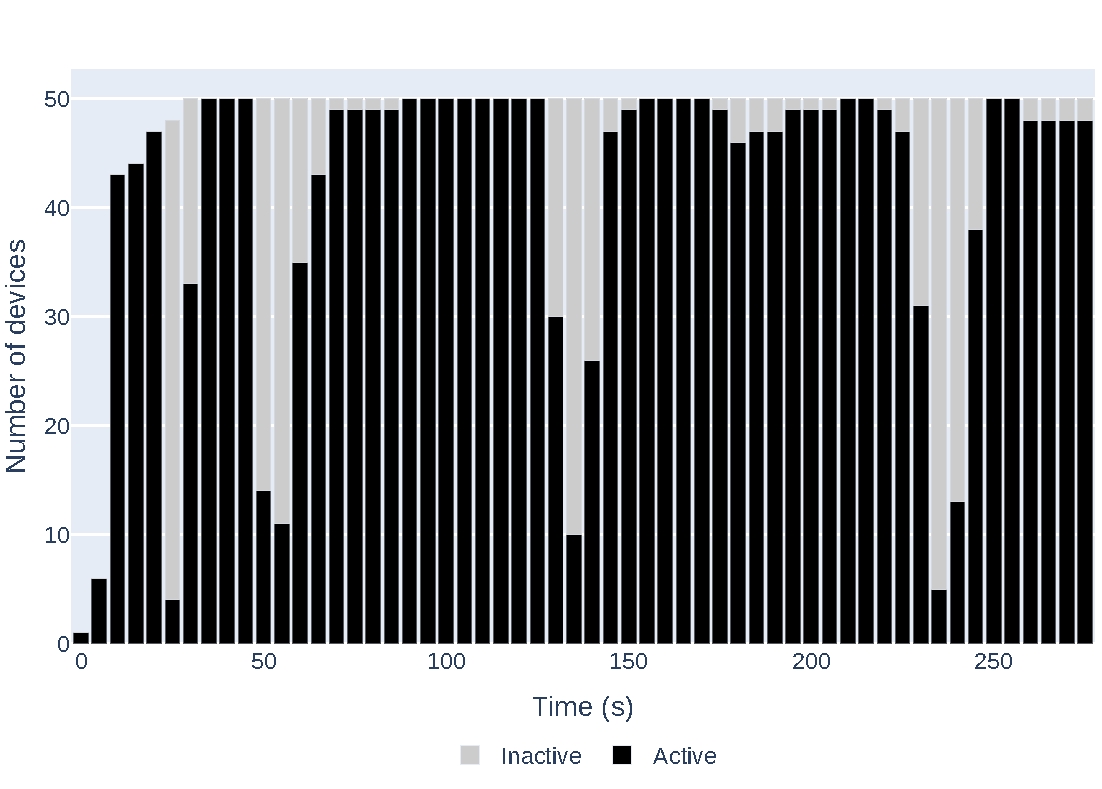
\includegraphics[width=\linewidth]{experiences/F-stress_test/status.pdf}
\caption[Number of devices active and inactive]{Number of devices active and inactive}\label{fig:stress_test_status}
\end{figure}

%%%%%%%%%%%%%%%%%%%%%%%%%%%%%%%%%%%%%%%%%%%%

\subsection{ES2: Experimental Tasks}\label{sec:discussion_scenario2}

As mentioned previously, several experiences were made to compare the developed solution to existing ones. To this end goal, a simple experiment of passing a message through several devices was implemented and the time the message takes to pass through all the devices was measured. The implementation of the scenario in the Node-RED tool is shown in \figureref{fig:scenario2_node_red}. The \textit{nothing} \textit{nodes} execution consists of only redirecting their input to their output. The message consisting of the current timestamp is inserted into the system by the \textit{inject} \textit{node} with user input, and the same message is showcased by the \textit{debug} node, the green one.

\begin{figure}[h]
\centering
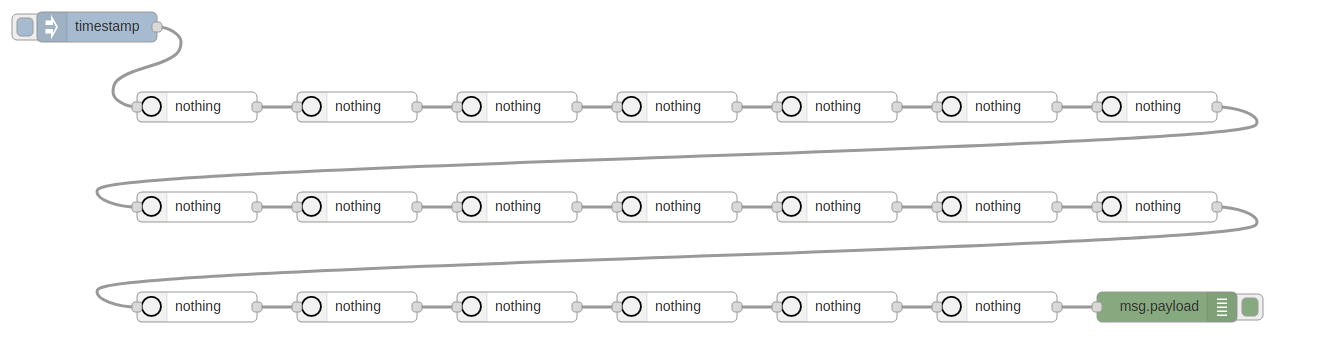
\includegraphics[width=\linewidth]{scenario2.png}
\caption[Node-RED implementation of scenario 2]{Node-RED implementation of scenario 2}\label{fig:scenario2_node_red}
\end{figure}

This same setup was replicated in several environments, as mentioned before. Each experiment was replicated 10 times, and the resulting time measurements are show in \tableref{tab:scenario2_table} and \figureref{fig:scenario2_candlestick}.

\captionsetup{belowskip=12pt,aboveskip=4pt}
\begin{table}[ht]
    \centering
    \resizebox{0.8\textwidth}{!}{%
    \begin{tabular}{ l  c  c  c  c }
        \toprule
        \textbf{Label} & \textbf{Min} & \textbf{Q2} & \textbf{Q3} & \textbf{Max}\\
        \midrule
        \textbf{ES2-A}: Node-RED original & 3 & 10 & 13.25 & 15 \\
        \textbf{ES2-B}: Node-RED + MQTT & 134 & 430.5 & 711.25 & 883 \\
        \textbf{ES2-C}: Node-RED modified + Dockers (same host) & 1217 & 1318 & 1573.75 & 1665 \\
        \textbf{ES2-D}: Node-RED modified + Dockers (different host) & 1445 & 2536 & 2708 & 3059 \\
        \textbf{ES2-E}: Physical + MQTT & 3616 & 4142 & 4372 & 4452 \\
        \textbf{ES2-F}: Node-RED modified + MQTT + Physical + Firmware & 4168 & 4569 & 5087.75 & 5940 \\
        \bottomrule
    \end{tabular}
    }
    \caption{Scenario 2 results}
    \label{tab:scenario2_table}
\end{table}{}

\begin{figure}[h]
\centering
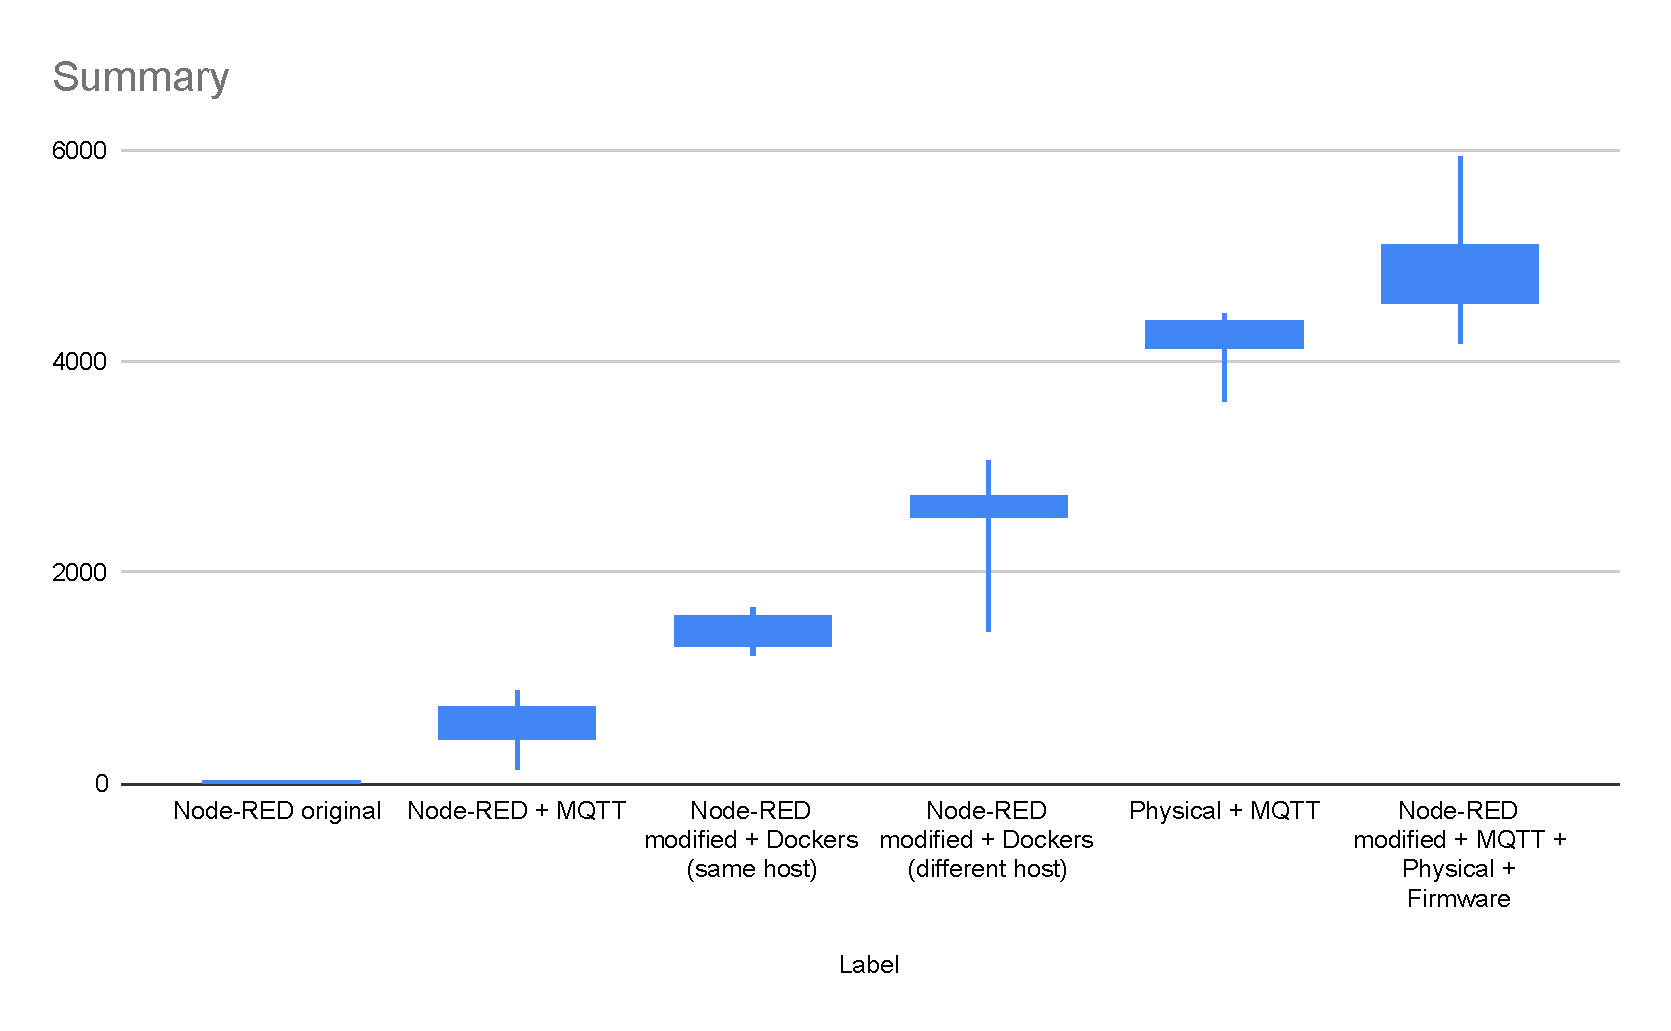
\includegraphics[width=\textwidth]{scenario2_graph.pdf}
\caption[ES2 results.]{ES2 results.}\label{fig:scenario2_candlestick}
\end{figure}

\figureref{fig:scenario2_candlestick} demonstrates that the developed solution is considerably less efficient in communicating message between nodes. However, given the other experiences, it is possible to conclude that this lack of efficiency is caused not by the firmware created but because of the stack of communication the message as to go through, as well as the nature of MicroPython. 

When the decentralization is applied inside Node-RED, without running any MicroPython, it is possible to see that the introduction of a Mosquitto broker running in the same host causes some latency. The introduction of Dockers running the firmware in the same host as the Node-RED instance and Mosquitto broker causes more latency, making it possible to conclude that MicroPython of the developed firmware also delay de communication. By repeating the same experience as before but with the Mosquitto broker in another machine, it is noticeable that the times are more spread out and the overall latency of the system is bigger. Given the stacks of Wi-Fi that the message as to go through, this result is logical.

Lastly, the experiment was repeated in physical devices, first by running a simple code in he MicroPython flashed devices and insertion of the message using the Mosquitto client, and second by using the whole developed system, with the modified Node-RED and firmware in the devices. The results allows us to conclude that the devices produce the worst time, but firmware developed introduces little latency, visible by the comparison of both their results.

It is possible to conclude that the developed solution's \textit{node} communication is slower than the original Node-RED mostly due to the nature of Wi-Fi communications and the MicroPython port used.

\section{Hypothesis Evaluation}\label{sec:evaluation_hypothesis}

This evaluation process aimed to prove the hypothesis presented in Section \ref{sec:main_hypothesis}.

Given the results of the experiments, it is possible to conclude that the system's implemented features are working, more specifically the decentralization of computation, handling of device's memory constraints and dynamic adaptation of the system. The attributes mentioned in \sectionref{sec:main_hypothesis} were evaluated, resulting in the following conclusions:

\begin{itemize}
    \item \textbf{Resilience}: The developed solution is moderately robust, handling device failures and memory constraints dynamically at run-time. However, there are some limitations to this robustness. As demonstrated in Section \ref{sec:experiment_f}, the system reaches a maximum point of adaptability when several devices fail and recover constantly.
    \item \textbf{Efficiency}: The developed solution is slower that the original Node-RED system. However, as demonstrated in \sectionref{sec:discussion_scenario2}, the increased latency is due to the introduced communication stack between \textit{nodes}, that changed from Javascript events into MQTT communications. This new way of communication in addition to the Wi-Fi stack and MicroPython firmware introduces latency. Despite this, the developed modules, such as the orchestrator and the device's firmware introduce little latency to the latency of the whole system.
    \item \textbf{Elasticity}: The solution handles a different number of devices, as it was demonstrated in the experiments from \sectionref{sec:scenarios_experiments}. It also handles the number of devices changes throughout the lifespan of the system, adapting the orchestration to the number of devices available.
\end{itemize}

In conclusion, the developed solution is more scalable than a centralized one, dealing with a dynamic number of devices while taking advantage of their computational capabilities. It is also robust to handle the failures and constraints of these devices. Lastly, the developed solution is not more efficient, but the its latency is due to factors external to the developed firmware. Since it is a decentralized solution, implementations with increased latency were made to enable communication between \textit{nodes}.

\section{Lessons Learned}\label{sec:evaluation_lessons_learned}

There were several changes made to the developed solution during the evaluation process. These changes were necessary to allow the capture of data that was later used to generate graphics and reach conclusions. The lessons learned during this process consisted in learning how to build a framework that supported sending and capture of data, as well as its aggregation and visualization. 

Each device was modified to allow them to send metrics to MQTT topics, which in turn were captured by a bridge that populated an InfluxDB database. This database supplied a Grafana dashboard, were the data from the evaluation was exported from. In addition to this, both the devices and Node-RED sent data to a Logstash, which supplied both a Kibana instance using Elastic Search. These logs were sometimes useful to understand the events happening in the devices and orchestrator in more complex experiments.

The setup necessary for this process required learning tools and modifying the developed solution. It was an iterative process in which the number of metrics captured increased each time an experiment was made. Due to this fact, the evaluation process took more time than was expected.

\section{Conclusions}\label{sec:evaluation_conclusions}

This Chapter presents the results from the evaluation process of the developed solution. \sectionref{sec:scenarios_experiments} starts by defining the scenarios and experiments that were used to test the tool and its compliance with the proposed requirements. \sectionref{sec:evaluation_discussion} analyzes the results from the experiments and reaches conclusions about the requirement each test was measuring. \sectionref{sec:evaluation_hypothesis} verifies if the data contrived from the evaluation process proves this dissertation hypothesis. Finally, \sectionref{sec:evaluation_lessons_learned} reflects on the lessons learned during the evaluation process. 

